\documentclass[11pt,twoside]{book}

%%Page Size (rev. 08/19/2016)
%\usepackage[inner=0.5in, outer=0.5in, top=0.5in, bottom=0.5in, papersize={6in,9in}, head=12pt, headheight=30pt, headsep=5pt]{geometry}
\usepackage[inner=0.5in, outer=0.5in, top=0.5in, bottom=0.5in, papersize={5.5in,8.5in}, head=12pt, headheight=30pt, headsep=5pt, footskip=20pt]{geometry}
%% width of textblock = 324 pt / 4.5in
%% A5 = 5.8 x 8.3 inches -- if papersize is A5, then margins should be [inner=0.75in, outer=0.55in, top=0.4in, bottom=0.4in]


%%Header (rev. 4/11/2011)
\usepackage{fancyhdr}
 \pagestyle{fancy}
\renewcommand{\chaptermark}[1]{\markboth{#1}{}}
\renewcommand{\sectionmark}[1]{\markright{#1}}
 \fancyhf{}
\fancyhead[LE,RO]{\thepage}
\fancyhead[CE]{\leftmark}
\fancyhead[CO]{\rightmark}

 \fancypagestyle{centernumber}{ %
\fancyhf{} % remove everything
\cfoot{\thepage}
\renewcommand{\headrulewidth}{0pt} % remove lines as well
\renewcommand{\footrulewidth}{0pt}
}

\fancypagestyle{plain}{%
\fancyhf{}    %pagestyle definition
\renewcommand{\headrulewidth}{0pt} % remove lines as well
\renewcommand{\footrulewidth}{0pt}
}






\usepackage[autocompile,allowdeprecated=false]{gregoriotex}
\usepackage{gregoriosyms}
\gresetgregoriofont[op]{greciliae}




%%Titles (rev. 9/4/2011) -- TOCLESS --- lets you have sections that don't appear in the table of contents

\setcounter{secnumdepth}{-1}
\setcounter{tocdepth}{1}

%%Variation 1.9.18 3:45 pm
\usepackage[compact,nobottomtitles*]{titlesec}
\titlespacing*{\chapter}{0pt}{-30pt}{0pt}
\titlespacing*{\section}{0pt}{*0}{*1}
\titlespacing*{\subsubsection}{0pt}{*0}{*0}
\titlespacing*{\subsubsubsection}{0pt}{10pt}{*0}
\titleformat{\part}{\normalfont\Huge\sc\center}{\thepart}{1em}{}
\titleformat{\chapter}{\normalfont\LARGE\sc\center}{\thechapter}{1em}{}
\titleformat{\section}{\normalfont\Large\sc\center}{\thesection}{1em}{}
\titleformat{\subsection}{\normalfont\fontsize{13}{15.6}\sc\center}{\thesubsection}{1em}{}
\titleformat{\subsubsection}{\normalfont\large\sc\center}{\thesubsubsection}{1em}{}
\titleformat{\paragraph}{\normalfont\normalsize\sc\center}{\thesubsubsection}{1em}{}

\newcommand{\nocontentsline}[3]{}
\newcommand{\tocless}[2]{\bgroup\let\addcontentsline=\nocontentsline#1{#2}\egroup} %% lets you have sections that don't appear in the table of contents


%%%

%%Index (rev. December 11, 2013)
\usepackage[nonewpage]{imakeidx}

\makeindex[name=Antiphons,title=Antiphons,columns=1]
\makeindex[name=Canticles,title=Canticles,columns=1]
\makeindex[name=Hymns,title=Hymns,columns=1]
\makeindex[name=Prayers,title=Prayers,columns=1]
\makeindex[name=Psalms,title=Psalms,columns=1]
\makeindex[name=Responsories,title=Responsories,columns=1]
\makeindex[name=Varia,title=Varia,columns=1]

\indexsetup{level=\section*,toclevel=section,noclearpage}

%\usepackage[indentunit=8pt,rule=.5pt,columns=2]{idxlayout}


%%Table of Contents (rev. May 16, 2011)

%\usepackage{multicol}
%\usepackage{ifthen}
%\usepackage[toc]{multitoc}

%% General settings (rev. January 19, 2015)

\usepackage{ulem}

\usepackage[latin,english]{babel}
\usepackage{lettrine}

\usepackage{paracol}

\usepackage{fontspec}

\setmainfont[Ligatures=TeX,BoldFont=MinionPro-Bold,ItalicFont=MinionPro-It, BoldItalicFont=MinionPro-BoldIt]{MinionPro-Regular-Modified.otf}


\usepackage{unicode-math}
\setmathfont{LatinModernMath-Regular}
\AtBeginDocument{\grelatexsimpledefbarredsymbol{V}{0.1em}{0.12em}{0.14em}{0.18em}}


%% Style for translation line
\grechangestyle{translation}{\fontsize{10}{10}\it\selectfont}
\grechangestyle{annotation}{\fontsize{10}{10}\selectfont}
\grechangestyle{commentary}{\textnormal\selectfont}
\gresetcustosalteration{invisible}

%\grechangedim{annotationseparation}{0.1cm}{scalable}

%\GreLoadSpaceConf{smith-four}

\frenchspacing

\usepackage{indentfirst} %%%indents first line after a section

\usepackage{graphicx}
%\usepackage{tocloft}

%%Hyperref (rev. August 20, 2011)
%\usepackage[colorlinks=false,hyperindex=true,bookmarks=true]{hyperref}
\usepackage{hyperref}
\hypersetup{pdftitle={Vesperale O.P. 2017}}
\hypersetup{pdfauthor={Order of Preachers}}
\hypersetup{pdfsubject={Liturgy}}
\hypersetup{pdfkeywords={Dominican, Liturgy, Order of Preachers, Dominican Rite, Liturgia Horarum, Divine Office}}

\newlength{\drop}



\begin{document}


%%%Initial Matter within Body (20 May 2011)
\raggedbottom

\newcommand{\lectio}[3]{%
  \makebox[0pt][l]{#1}%
  \makebox[\textwidth][c]{#2}%
  \makebox[0pt][r]{\normalsize{\textnormal{#3}}}}


%%Combination

%%Combination
\begin{titlepage}
    \drop=0.1\textheight
    \centering
    \vspace*{\baselineskip}
   % \rule{\textwidth}{1.6pt}\vspace*{-\baselineskip}\vspace*{2pt}
    %\rule{\textwidth}{0.4pt}\\[\baselineskip]
    {\fontsize{50pt}{50pt}\selectfont COMPLINE \\ \vspace{10pt} \large \textsc{with elements proper to the}\\\vspace{10pt} \fontsize{20pt}{20pt}\selectfont  \textsc{Order of Friars Preachers}
   % \rule{\textwidth}{0.4pt}\vspace*{-\baselineskip}\vspace{3.2pt}
    %\rule{\textwidth}{1.6pt}\\[\baselineskip]

    \vspace*{100pt}

    \begin{figure}[h]
\centering
      
\includegraphics[width=1.75in]{op-shield.jpg} %
    \end{figure}


    \vfill
    {\fontsize{13pt}{20pt}\selectfont \textsc{New York} \par \textsc{Atelier St. Jacques} \par \scshape{2018} \par }}
  \end{titlepage}





  %%Combination
  \tableofcontents
  \thispagestyle{centernumber} \chapter{Psalter} \cleardoublepage
  \thispagestyle{centernumber} \section{Sunday or Solemnity after First Vespers}
                \par \lettrine[lines=3]{O}{} Sacred Banquet, in which Christ becomes our food, the memory of his passion is celebrated, the soul is filled with grace, and the pledge of future glory is given to us. \par \vspace{5pt} \Vbar. You gave them bread from heaven. \par \Rbar. Containing every blessing. \vspace{5pt} \par \lettrine[lines=2]{L}{}et us pray. O God, who in this wonderful sacrament have left us a memorial of your Passion, grant us, we pray, so to revere the sacred mysteries of your Body and Blood that we may always experience in ourselves the fruits of your redemption. Through Christ our Lord. \Rbar. Amen. \par \vspace{5pt}
    \emph{Stand}  \index[Varia]{O God come to my assistance} \label{O God come to my assistance (Varia)} \grecommentary[0pt]{} \grechangestyle{initial}{\fontsize{1}{1}\selectfont} \grechangestyle{initial}{\fontsize{36}{36}\selectfont} \grechangedim{maxbaroffsettextleft@nobar}{12 cm}{scalable} \grechangedim{spaceabovelines}{0.4cm}{scalable} \gresetlyriccentering{syllable}  \grechangedim{maxbaroffsettextleft}{0 cm}{scalable} \gregorioscore{chants/misc.o_god_come-psj}
   \subsubsection{Examination of Conscience} \emph{Kneel}            \par \lettrine[lines=3]{I}{} confess to Almighty God, to Blessed Mary ever-Virgin, to Blessed Dominic, our father, to all the saints, and to you, my brothers (and sisters), that I have sinned through my own fault, in my thoughts and in my words, in what I have done and in what I have failed to do. I beseech you to pray for me. \par \Vbar. May Almighty God have mercy on us, forgive us our sins, keep us safe and strengthen us in every good work, and bring us to everlasting life. \par \Rbar. Amen.
   \subsubsection{Hymnus}  \greannotation{VIII} \index[Hymns]{Te lucis ante terminum (Sundays in Ordinary Time after First Vespers)} \label{Te lucis ante terminum (Sundays in Ordinary Time after First Vespers) (Hymnus)} \grecommentary[0pt]{} \grechangestyle{initial}{\fontsize{1}{1}\selectfont} \grechangestyle{initial}{\fontsize{36}{36}\selectfont} \grechangedim{maxbaroffsettextleft@nobar}{12 cm}{scalable} \grechangedim{spaceabovelines}{0.5cm}{scalable} \gresetlyriccentering{vowel}   \gregorioscore{chants/hy--te_lucis--sunday--first-vespers}    \newpage
   \subsubsection{Hymn}  \greannotation{VIII} \index[Hymns]{To you before the close of day (Sundays in Ordinary Time after First Vespers)} \label{To you before the close of day (Sundays in Ordinary Time after First Vespers) (Hymn)} \grecommentary[0pt]{} \grechangestyle{initial}{\fontsize{1}{1}\selectfont} \grechangestyle{initial}{\fontsize{36}{36}\selectfont} \grechangedim{maxbaroffsettextleft@nobar}{12 cm}{scalable} \grechangedim{spaceabovelines}{0.5cm}{scalable} \gresetlyriccentering{syllable}   \gregorioscore{chants/hy--te_lucis--sunday--first-vespers.english}    \newpage
   \subsubsection{Antiphon}  \greannotation{VIII} \index[Antiphons]{Have mercy Lord} \label{Have mercy Lord (Antiphon)} \grecommentary[0pt]{Ps 4:2} \grechangestyle{initial}{\fontsize{1}{1}\selectfont} \grechangestyle{initial}{\fontsize{36}{36}\selectfont} \grechangedim{maxbaroffsettextleft@nobar}{12 cm}{scalable} \grechangedim{spaceabovelines}{0.5cm}{scalable} \gresetlyriccentering{syllable}  \grechangedim{maxbaroffsettextleft}{0 cm}{scalable} \gregorioscore{chants/gethsemane01saturday1stvespers1.have.mercy}  \grechangedim{maxbaroffsettextleft}{0.6 cm}{scalable}  \vspace{5pt} \hfill \emph{During the Easter Season:} Alleluia, p. \pageref{Alleluia, alleluia, alleluia (Psalm Antiphon)}.
   \subsubsection{Psalm 4} \paragraph{Thanksgiving}  \index[Psalms]{Psalm 4} \label{Psalm 4 (Psalm)} \noindent \emph{The resurrection of Christ was God’s supreme and wholly marvelous work \linebreak \hspace*{0pt}\hfill \emph{(Saint Augustine).}}        \vspace{5pt} \par \noindent  When I call, answer me, O God of justice;~\GreStar{}~\nopagebreak

from anguish you released me, have mercy and hear me!

\noindent O men, how long will your hearts be closed,~\GreStar{}~\nopagebreak

will you love what is futile and seek what is false?

\noindent It is the Lord who grants favors to those whom he loves;~\GreStar{}~\nopagebreak

the Lord hears me whenever I call him.

\noindent Fear him; do not sin: ponder on your bed and be still.~\GreStar{}~\nopagebreak

Make justice your sacrifice, and trust in the Lord.

\noindent ``What can bring us happiness?" many say.~\GreStar{}~\nopagebreak

Let the light of your face shine on us, O Lord.

\noindent You have put into my heart a greater joy~\GreStar{}~\nopagebreak

than they have from abundance of corn and new wine.

\noindent I will lie down in peace and sleep comes at once~\GreStar{}~\nopagebreak

for you alone, Lord, make me dwell in safety.

\noindent Glory to the Father, and to the Son,~\GreStar{}~\nopagebreak

and to the Holy Spirit:

\noindent as it was in the beginning, is now,~\GreStar{}~\nopagebreak

and will be for ever. Amen.
    \newpage
   \subsubsection{Antiphon}  \greannotation{VI} \index[Antiphons]{In the silent hours} \label{In the silent hours (Antiphon)} \grecommentary[0pt]{Ps 133:2} \grechangestyle{initial}{\fontsize{1}{1}\selectfont} \grechangestyle{initial}{\fontsize{36}{36}\selectfont} \grechangedim{maxbaroffsettextleft@nobar}{12 cm}{scalable} \grechangedim{spaceabovelines}{0.5cm}{scalable} \gresetlyriccentering{syllable}  \grechangedim{maxbaroffsettextleft}{0 cm}{scalable} \gregorioscore{chants/gethsemane01saturday1stvespers2.in.the.silent}  \grechangedim{maxbaroffsettextleft}{0.6 cm}{scalable}  \vspace{5pt} \hfill \emph{During the Easter Season, the second antiphon is omitted.}
   \subsubsection{Psalm 133 (134)} \paragraph{Evening prayer in the Temple}  \index[Psalms]{Psalm 133 (134)} \label{Psalm 133 (134) (Psalm)} \noindent \emph{Praise our God, all you his servants, you who fear him, small and great \linebreak \hspace*{0pt}\hfill \emph{(Revelation 19:5).}}        \vspace{5pt} \par \noindent O come, bless the Lord,~\GreStar{}~\nopagebreak

all you who serve the Lord,

\noindent who stand in the house of the Lord,~\GreStar{}~\nopagebreak

in the courts of the house of our God.

\noindent Lift up your hands to the holy place~\GreStar{}~\nopagebreak

and bless the Lord through the night.

\noindent May the Lord bless you from Zion,~\GreStar{}~\nopagebreak

he who made both heaven and earth.

\noindent Glory to the Father, and to the Son,~\GreStar{}~\nopagebreak

and to the Holy Spirit:

\noindent as it was in the beginning, is now,~\GreStar{}~\nopagebreak

and will be for ever. Amen.
    \newpage
   \subsubsection{\lectio{}{Reading}{Dt 6:4-7}}             \lettrine[loversize=0.15,lines=2]{H}{}ear, O Israel! The Lord is our God, the Lord alone! Therefore, you shall love the Lord, your God, with all your heart, and with all your soul, and with all your strength. Take to heart these words which I enjoin on you today. Drill them into your children. Speak of them at home and abroad, whether you are busy or at rest.

   \subsubsection{Seasonal and Festal Responsories}             Solemnities in Ordinary Time: \pageref{In manus tuas ... alleluia (Responsorium brevis)} or \pageref{Into your hands ... alleluia (Short responsory)}.

Christmas: \pageref{In manus tuas ... alleluia (Responsorium brevis)} or \pageref{Into your hands ... alleluia (Short responsory)}.

Lent and Holy Week: \pageref{Media vita (Responsorium prolixa)}.

Triduum: \pageref{Christus factus est (Responsorium)}.

Easter Octave: \pageref{Haec dies (Responsorium Prolixa)}, \pageref{This is the day (Dominican) (Responsorium (Dominican))}, or \pageref{This is the day (Gethsemani) (Responsorium (Gethsemani))}.

Easter Season: \pageref{In manus tuas ... alleluia (Responsorium brevis)} or \pageref{Into your hands ... alleluia (Short responsory)}.
   \subsubsection{Seasonal and Festal Canticles}             Christmas Eve: \pageref{Ecce completa (Antiphona ad Nunc dimittis)}.

Christmas to Epiphany: \pageref{Alleluia Verbum caro (Antiphona ad Nunc dimittis)}.

Epiphany: \pageref{Alleluia Omnes de Saba (Antiphona ad Nunc dimittis)}.

First and Second Weeks of Lent: \pageref{Evigila (Antiphona ad Nunc dimittis)}.

Third Week of Lent until the Paschal Triduum: \pageref{O Rex (Antiphona ad Nunc dimittis)}.

Easter to Ascension: \pageref{Alleluia Resurrexit (Antiphona ad Nunc dimittis)}.

Ascension to Pentecost: \pageref{Alleluia Ascendens (Antiphona ad Nunc dimittis)}.

Pentecost: \pageref{Alleluia Spiritus (Antiphona ad Nunc dimittis)}.

\vspace{5pt}

Presentation of the Lord: \pageref{Nunc dimittis (Antiphona ad Nunc dimittis)}.

Annunciation of the Lord: \pageref{Ecce ancilla Domini (Antiphona ad Nunc dimittis)}.

Most Holy Body and Blood of Christ: \pageref{Alleluia Panis (Antiphona ad Nunc dimittis)}.

Most Sacred Heart of Jesus: \pageref{Alleluia Haurietis (Antiphona ad Nunc dimittis)}.

Feasts of the Blessed Virgin Mary: \pageref{Corde et animo (Antiphona ad Nunc dimittis)} or \pageref{Sub tuum (Antiphona ad Nunc dimittis)}.
    \newpage
   \subsubsection{Responsorium brevis}  \greannotation{IV} \index[Responsories]{In manus tuas} \label{In manus tuas (Responsorium brevis)} \grecommentary[0pt]{Ps 30:6} \gresetinitiallines{1} \grechangestyle{initial}{\fontsize{36}{36}\selectfont} \grechangedim{maxbaroffsettextleft@nobar}{12 cm}{scalable} \grechangedim{spaceabovelines}{0.4cm}{scalable} \gresetlyriccentering{vowel}  \grechangedim{maxbaroffsettextleft}{0 cm}{scalable} \gregorioscore{chants/rb--in_manus}  \grechangedim{maxbaroffsettextleft}{0.6 cm}{scalable}
   \subsubsection{Short responsory}  \greannotation{VI} \index[Responsories]{Into your hands} \label{Into your hands (Short responsory)} \grecommentary[0pt]{Ps 30:6} \gresetinitiallines{1} \grechangestyle{initial}{\fontsize{36}{36}\selectfont} \grechangedim{maxbaroffsettextleft@nobar}{12 cm}{scalable} \grechangedim{spaceabovelines}{0.4cm}{scalable} \gresetlyriccentering{syllable}  \grechangedim{maxbaroffsettextleft}{0 cm}{scalable} \gregorioscore{chants/rb--into.your.hands}  \grechangedim{maxbaroffsettextleft}{0.6 cm}{scalable}  \newpage
   \subsubsection{Antiphona ad Nunc dimittis}  \greannotation{III a} \index[Antiphons]{Salva nos} \label{Salva nos (Antiphona ad Nunc dimittis)} \grecommentary[3pt]{Ecclesia} \gresetinitiallines{1} \grechangestyle{initial}{\fontsize{36}{36}\selectfont} \grechangedim{maxbaroffsettextleft@nobar}{12 cm}{scalable} \grechangedim{spaceabovelines}{0.5cm}{scalable} \gresetlyriccentering{vowel}   \gregorioscore{chants/an--salva_nos--dominican}
   \subsubsection{Canticum Evangelicum} \paragraph{Christus lumen gentium et gloria Israel} \greannotation{III a} \index[Canticles]{Nunc dimitis 3a} \label{Nunc dimitis 3a (Canticum Evangelicum)} \grecommentary[3pt]{Lc 2:29-32} \gresetinitiallines{1} \grechangestyle{initial}{\fontsize{36}{36}\selectfont} \grechangedim{maxbaroffsettextleft@nobar}{12 cm}{scalable} \grechangedim{spaceabovelines}{0.5cm}{scalable} \gresetlyriccentering{vowel}   \gregorioscore{chants/nunc_dimitis3a}
   \subsubsection{Antiphon for the Canticle of Simeon}  \greannotation{III a} \index[Antiphons]{Salva nos} \label{Salva nos (Antiphon for the Canticle of Simeon)} \grecommentary[5pt]{Ecclesia} \gresetinitiallines{1} \grechangestyle{initial}{\fontsize{36}{36}\selectfont} \grechangedim{maxbaroffsettextleft@nobar}{0pt}{scalable} \grechangedim{spaceabovelines}{0.5cm}{scalable} \gresetlyriccentering{vowel}  \grechangedim{maxbaroffsettextleft}{0 cm}{scalable} \gregorioscore{chants/an--protect.us.lord}  \grechangedim{maxbaroffsettextleft}{0.6 cm}{scalable}
   \subsubsection{Canticle of Simeon: Lk 2:29-32} \paragraph{Christ is the light of the nations and the glory of Israel}  \index[Canticles]{Canticle of Simeon: Lk 2:29-32} \label{Canticle of Simeon: Lk 2:29-32 (Gospel Canticle)}         \vspace{5pt} \par \lettrine[loversize=0.15,lines=2]{L}{}ord, now you let your servant go in peace;~$\star$~\nopagebreak

\hspace{2pt} your word has been fulfilled:

\noindent my own eyes have seen the salvation~$\star$~\nopagebreak

which you have prepared in the sight of every people:

\noindent a light to reveal you to the nations~$\star$~\nopagebreak

and the glory of your people Israel.

\noindent Glory to the Father, and to the Son,~$\star$~\nopagebreak

and to the Holy Spirit:

\noindent as it was in the beginning, is now,~$\star$~\nopagebreak

and will be for ever. Amen.
    \newpage

   \subsubsection{Concluding Prayer}   \index[Prayers]{Lord, be with us throughout this night} \label{Lord, be with us throughout this night (Concluding Prayer)}         \lettrine[loversize=0.15,lines=2]{L}{}ord,
be with us throughout this night.
When day comes may we rise from sleep
to rejoice in the resurrection of your Christ,
who lives and reigns for ever and ever.
\par \Rbar.~Amen.

   \subsubsection{Concluding Prayer} \emph{On solemnities that do not occur on Sunday:}  \index[Prayers]{Lord, we beg you to visit this house} \label{Lord, we beg you to visit this house (Concluding Prayer)}         \lettrine[loversize=0.15,lines=2]{L}{}ord, we beg you to visit this house and banish from it all the deadly power of the enemy. May your holy angels dwell here to keep us in peace, and may your blessing be upon us always. We ask this through Christ our Lord.
\par \Rbar. Amen.

   \subsubsection{Blessing}             \lettrine[loversize=0.15,lines=2]{M}{}ay the all-powerful Lord grant us a restful night and a peaceful death. \Rbar. Amen.    \newpage

  \thispagestyle{centernumber} \section{Sunday or Solemnity after Second Vespers}
                \par \lettrine[lines=3]{O}{} Sacred Banquet, in which Christ becomes our food, the memory of his passion is celebrated, the soul is filled with grace, and the pledge of future glory is given to us. \par \vspace{5pt} \Vbar. You gave them bread from heaven. \par \Rbar. Containing every blessing. \vspace{5pt} \par \lettrine[lines=2]{L}{}et us pray. O God, who in this wonderful sacrament have left us a memorial of your Passion, grant us, we pray, so to revere the sacred mysteries of your Body and Blood that we may always experience in ourselves the fruits of your redemption. Through Christ our Lord. \Rbar. Amen. \par \vspace{5pt}
    \emph{Stand}  \index[Varia]{O God come to my assistance} \label{O God come to my assistance (Varia)} \grecommentary[0pt]{} \grechangestyle{initial}{\fontsize{1}{1}\selectfont} \grechangestyle{initial}{\fontsize{36}{36}\selectfont} \grechangedim{maxbaroffsettextleft@nobar}{12 cm}{scalable} \grechangedim{spaceabovelines}{0.4cm}{scalable} \gresetlyriccentering{syllable}  \grechangedim{maxbaroffsettextleft}{0 cm}{scalable} \gregorioscore{chants/misc.o_god_come-psj}
   \subsubsection{Examination of Conscience} \emph{Kneel}            \par \lettrine[lines=3]{I}{} confess to Almighty God, to Blessed Mary ever-Virgin, to Blessed Dominic, our father, to all the saints, and to you, my brothers (and sisters), that I have sinned through my own fault, in my thoughts and in my words, in what I have done and in what I have failed to do. I beseech you to pray for me. \par \Vbar. May Almighty God have mercy on us, forgive us our sins, keep us safe and strengthen us in every good work, and bring us to everlasting life. \par \Rbar. Amen.
   \subsubsection{Hymnus}  \greannotation{VIII} \index[Hymns]{Te lucis ante terminum (Sundays in Ordinary Time after Second Vespers)} \label{Te lucis ante terminum (Sundays in Ordinary Time after Second Vespers) (Hymnus)} \grecommentary[0pt]{} \grechangestyle{initial}{\fontsize{1}{1}\selectfont} \grechangestyle{initial}{\fontsize{36}{36}\selectfont} \grechangedim{maxbaroffsettextleft@nobar}{12 cm}{scalable} \grechangedim{spaceabovelines}{0.5cm}{scalable} \gresetlyriccentering{vowel}   \gregorioscore{chants/hy--te_lucis--sunday--second-vespers}    \newpage
   \subsubsection{Hymn}  \greannotation{VIII} \index[Hymns]{To you before the close of day (Sundays in Ordinary Time after Second Vespers)} \label{To you before the close of day (Sundays in Ordinary Time after Second Vespers) (Hymn)} \grecommentary[0pt]{} \grechangestyle{initial}{\fontsize{1}{1}\selectfont} \grechangestyle{initial}{\fontsize{36}{36}\selectfont} \grechangedim{maxbaroffsettextleft@nobar}{12 cm}{scalable} \grechangedim{spaceabovelines}{0.5cm}{scalable} \gresetlyriccentering{syllable}   \gregorioscore{chants/hy--te_lucis--sunday--second-vespers.english}    \newpage
   \subsubsection{Antiphon}  \greannotation{V} \index[Antiphons]{Night holds no terrors} \label{Night holds no terrors (Antiphon)} \grecommentary[3pt]{Cf. Ps 90:3, 4} \grechangestyle{initial}{\fontsize{1}{1}\selectfont} \grechangestyle{initial}{\fontsize{36}{36}\selectfont} \grechangedim{maxbaroffsettextleft@nobar}{12 cm}{scalable} \grechangedim{spaceabovelines}{0.5cm}{scalable} \gresetlyriccentering{syllable}  \grechangedim{maxbaroffsettextleft}{0 cm}{scalable} \gregorioscore{chants/gethsemane02sunday2vespers.night.holds}  \grechangedim{maxbaroffsettextleft}{0.6 cm}{scalable}  \vspace{5pt} \hfill \emph{During the Easter Season:} Alleluia, p. \pageref{Alleluia, alleluia, alleluia (Psalm Antiphon)}.
   \subsubsection{Psalm 90 (91)} \paragraph{Safe in God’s sheltering care}  \index[Psalms]{Psalm 90 (91)} \label{Psalm 90 (91) (Psalm)} \noindent \emph{I have given you the power to tread upon serpents and scorpions \emph{(Luke 10:19).}}        \vspace{5pt} \par \noindent He who dwells in the shelter of the Most High~$\star$~\nopagebreak

and abides in the shade of the Almighty

\noindent says to the Lord: ``My refuge,~$\star$~\nopagebreak

my stronghold, my God in whom I trust!"

\noindent It is he who will free you from the snare~$\star$~\nopagebreak

of the fowler who seeks to destroy you;

\noindent he will conceal you with his pinions~$\star$~\nopagebreak

and under his wings you will find refuge.

\noindent You will not fear the terror of the night~$\star$~\nopagebreak

nor the arrow that flies by day,

\noindent nor the plague that prowls in the darkness~$\star$~\nopagebreak

nor the scourge that lays waste at noon.

\noindent A thousand may fall at your side,~$\star$~\nopagebreak

ten thousand fall at your right,

\noindent you, it will never approach;~$\star$~\nopagebreak

his faithfulness is buckler and shield.

\noindent Your eyes have only to look~$\star$~\nopagebreak

to see how the wicked are repaid,

\noindent you who have said: ``Lord, my refuge!"~$\star$~\nopagebreak

and have made the Most High your dwelling.

\noindent Upon you no evil shall fall,~$\star$~\nopagebreak

no plague approach where you dwell.

\noindent For you has he commanded his angels,~$\star$~\nopagebreak

to keep you in all your ways.

\noindent They shall bear you upon their hands~$\star$~\nopagebreak

lest you strike your foot against a stone.

\noindent On the lion and the viper you will tread~$\star$~\nopagebreak

and trample the young lion and the dragon.

\noindent Since he clings to me in love, I will free him;~$\star$~\nopagebreak

protect him for he knows my name.

\noindent When he calls I shall answer: ``I am with you,"~$\star$~\nopagebreak

I will save him in distress and give him glory.

\noindent With length of life I will content him;~$\star$~\nopagebreak

I shall let him see my saving power.

\noindent Glory to the Father, and to the Son,~$\star$~\nopagebreak

and to the Holy Spirit:

\noindent as it was in the beginning, is now,~$\star$~\nopagebreak

and will be for ever. Amen.
    \newpage
   \subsubsection{\lectio{}{Reading}{Rev 22:4-5}}             \lettrine[loversize=0.15,lines=2]{T}{}hey shall see the Lord face to face and bear his name on their foreheads. The night shall be no more. They will need no light from lamps or the sun, for the Lord God shall give them light, and they shall reign forever.
   \subsubsection{Seasonal and Festal Responsories}             Solemnities in Ordinary Time: \pageref{In manus tuas ... alleluia (Responsorium brevis)} or \pageref{Into your hands ... alleluia (Short responsory)}.

Christmas: \pageref{In manus tuas ... alleluia (Responsorium brevis)} or \pageref{Into your hands ... alleluia (Short responsory)}.

Lent and Holy Week: \pageref{Media vita (Responsorium prolixa)}.

Triduum: \pageref{Christus factus est (Responsorium)}.

Easter Octave: \pageref{Haec dies (Responsorium Prolixa)}, \pageref{This is the day (Dominican) (Responsorium (Dominican))}, or \pageref{This is the day (Gethsemani) (Responsorium (Gethsemani))}.

Easter Season: \pageref{In manus tuas ... alleluia (Responsorium brevis)} or \pageref{Into your hands ... alleluia (Short responsory)}.
   \subsubsection{Seasonal and Festal Canticles}             Christmas: \pageref{Alleluia Verbum caro (Antiphona ad Nunc dimittis)}.

Epiphany: \pageref{Alleluia Omnes de Saba (Antiphona ad Nunc dimittis)}.

First and Second Weeks of Lent: \pageref{Evigila (Antiphona ad Nunc dimittis)}.

Third Week of Lent until the Paschal Triduum: \pageref{O Rex (Antiphona ad Nunc dimittis)}.

Easter to Ascension: \pageref{Alleluia Resurrexit (Antiphona ad Nunc dimittis)}.

Ascension to Pentecost: \pageref{Alleluia Ascendens (Antiphona ad Nunc dimittis)}.

Pentecost: \pageref{Alleluia Spiritus (Antiphona ad Nunc dimittis)}.

\vspace{5pt}

Presentation of the Lord: \pageref{Nunc dimittis (Antiphona ad Nunc dimittis)}.

Annunciation of the Lord: \pageref{Ecce ancilla Domini (Antiphona ad Nunc dimittis)}.

Most Holy Body and Blood of Christ: \pageref{Alleluia Panis (Antiphona ad Nunc dimittis)}.

Most Sacred Heart of Jesus: \pageref{Alleluia Haurietis (Antiphona ad Nunc dimittis)}.

Feasts of the Blessed Virgin Mary: \pageref{Corde et animo (Antiphona ad Nunc dimittis)} or \pageref{Sub tuum (Antiphona ad Nunc dimittis)}.
    \newpage
   \subsubsection{Responsorium brevis}  \greannotation{IV} \index[Responsories]{In manus tuas} \label{In manus tuas (Responsorium brevis)} \grecommentary[0pt]{Ps 30:6} \gresetinitiallines{1} \grechangestyle{initial}{\fontsize{36}{36}\selectfont} \grechangedim{maxbaroffsettextleft@nobar}{12 cm}{scalable} \grechangedim{spaceabovelines}{0.4cm}{scalable} \gresetlyriccentering{vowel}  \grechangedim{maxbaroffsettextleft}{0 cm}{scalable} \gregorioscore{chants/rb--in_manus}  \grechangedim{maxbaroffsettextleft}{0.6 cm}{scalable}
   \subsubsection{Short responsory}  \greannotation{VI} \index[Responsories]{Into your hands} \label{Into your hands (Short responsory)} \grecommentary[0pt]{Ps 30:6} \gresetinitiallines{1} \grechangestyle{initial}{\fontsize{36}{36}\selectfont} \grechangedim{maxbaroffsettextleft@nobar}{12 cm}{scalable} \grechangedim{spaceabovelines}{0.4cm}{scalable} \gresetlyriccentering{syllable}  \grechangedim{maxbaroffsettextleft}{0 cm}{scalable} \gregorioscore{chants/rb--into.your.hands}  \grechangedim{maxbaroffsettextleft}{0.6 cm}{scalable}  \newpage
   \subsubsection{Antiphona ad Nunc dimittis}  \greannotation{III a} \index[Antiphons]{Salva nos} \label{Salva nos (Antiphona ad Nunc dimittis)} \grecommentary[3pt]{Ecclesia} \gresetinitiallines{1} \grechangestyle{initial}{\fontsize{36}{36}\selectfont} \grechangedim{maxbaroffsettextleft@nobar}{12 cm}{scalable} \grechangedim{spaceabovelines}{0.5cm}{scalable} \gresetlyriccentering{vowel}   \gregorioscore{chants/an--salva_nos--dominican}
   \subsubsection{Canticum Evangelicum} \paragraph{Christus lumen gentium et gloria Israel} \greannotation{III a} \index[Canticles]{Nunc dimitis 3a} \label{Nunc dimitis 3a (Canticum Evangelicum)} \grecommentary[3pt]{Lc 2:29-32} \gresetinitiallines{1} \grechangestyle{initial}{\fontsize{36}{36}\selectfont} \grechangedim{maxbaroffsettextleft@nobar}{12 cm}{scalable} \grechangedim{spaceabovelines}{0.5cm}{scalable} \gresetlyriccentering{vowel}   \gregorioscore{chants/nunc_dimitis3a}
   \subsubsection{Antiphon for the Canticle of Simeon}  \greannotation{III a} \index[Antiphons]{Salva nos} \label{Salva nos (Antiphon for the Canticle of Simeon)} \grecommentary[5pt]{Ecclesia} \gresetinitiallines{1} \grechangestyle{initial}{\fontsize{36}{36}\selectfont} \grechangedim{maxbaroffsettextleft@nobar}{0pt}{scalable} \grechangedim{spaceabovelines}{0.5cm}{scalable} \gresetlyriccentering{vowel}  \grechangedim{maxbaroffsettextleft}{0 cm}{scalable} \gregorioscore{chants/an--protect.us.lord}  \grechangedim{maxbaroffsettextleft}{0.6 cm}{scalable}
   \subsubsection{Canticle of Simeon: Lk 2:29-32} \paragraph{Christ is the light of the nations and the glory of Israel}  \index[Canticles]{Canticle of Simeon: Lk 2:29-32} \label{Canticle of Simeon: Lk 2:29-32 (Gospel Canticle)}         \vspace{5pt} \par \lettrine[loversize=0.15,lines=2]{L}{}ord, now you let your servant go in peace;~$\star$~\nopagebreak

\hspace{2pt} your word has been fulfilled:

\noindent my own eyes have seen the salvation~$\star$~\nopagebreak

which you have prepared in the sight of every people:

\noindent a light to reveal you to the nations~$\star$~\nopagebreak

and the glory of your people Israel.

\noindent Glory to the Father, and to the Son,~$\star$~\nopagebreak

and to the Holy Spirit:

\noindent as it was in the beginning, is now,~$\star$~\nopagebreak

and will be for ever. Amen.
    \newpage

   \subsubsection{Concluding Prayer}   \index[Prayers]{Lord, we have celebrated today} \label{Lord, we have celebrated today (Concluding Prayer)}         \lettrine[loversize=0.15,lines=2]{L}{}ord,
we have celebrated today
the mystery of the rising of Christ to new life.
May we now rest in your peace,
safe from all that could harm us,
and rise again refreshed and joyful,
to praise you throughout another day.
We ask this through Christ our Lord.
\par \Rbar. Amen.

   \subsubsection{Concluding Prayer} \emph{On solemnities that do not occur on Sunday:}  \index[Prayers]{Lord, we beg you to visit this house} \label{Lord, we beg you to visit this house (Concluding Prayer)}         \lettrine[loversize=0.15,lines=2]{L}{}ord, we beg you to visit this house and banish from it all the deadly power of the enemy. May your holy angels dwell here to keep us in peace, and may your blessing be upon us always. We ask this through Christ our Lord.
\par \Rbar. Amen.

   \subsubsection{Blessing}             \lettrine[loversize=0.15,lines=2]{M}{}ay the all-powerful Lord grant us a restful night and a peaceful death. \Rbar. Amen.    \newpage

  \thispagestyle{centernumber} \section{Monday}
                \par \lettrine[lines=3]{O}{} Sacred Banquet, in which Christ becomes our food, the memory of his passion is celebrated, the soul is filled with grace, and the pledge of future glory is given to us. \par \vspace{5pt} \Vbar. You gave them bread from heaven. \par \Rbar. Containing every blessing. \vspace{5pt} \par \lettrine[lines=2]{L}{}et us pray. O God, who in this wonderful sacrament have left us a memorial of your Passion, grant us, we pray, so to revere the sacred mysteries of your Body and Blood that we may always experience in ourselves the fruits of your redemption. Through Christ our Lord. \Rbar. Amen. \par \vspace{5pt}
    \emph{Stand}  \index[Varia]{O God come to my assistance} \label{O God come to my assistance (Varia)} \grecommentary[0pt]{} \grechangestyle{initial}{\fontsize{1}{1}\selectfont} \grechangestyle{initial}{\fontsize{36}{36}\selectfont} \grechangedim{maxbaroffsettextleft@nobar}{12 cm}{scalable} \grechangedim{spaceabovelines}{0.4cm}{scalable} \gresetlyriccentering{syllable}  \grechangedim{maxbaroffsettextleft}{0 cm}{scalable} \gregorioscore{chants/misc.o_god_come-psj}
   \subsubsection{Examination of Conscience} \emph{Kneel}            \par \lettrine[lines=3]{I}{} confess to Almighty God, to Blessed Mary ever-Virgin, to Blessed Dominic, our father, to all the saints, and to you, my brothers (and sisters), that I have sinned through my own fault, in my thoughts and in my words, in what I have done and in what I have failed to do. I beseech you to pray for me. \par \Vbar. May Almighty God have mercy on us, forgive us our sins, keep us safe and strengthen us in every good work, and bring us to everlasting life. \par \Rbar. Amen.
   \subsubsection{Hymnus}  \greannotation{VIII} \index[Hymns]{Te lucis ante terminum (Weekdays in Ordinary Time and Advent)} \label{Te lucis ante terminum (Weekdays in Ordinary Time and Advent) (Hymnus)} \grecommentary[0pt]{} \grechangestyle{initial}{\fontsize{1}{1}\selectfont} \grechangestyle{initial}{\fontsize{36}{36}\selectfont} \grechangedim{maxbaroffsettextleft@nobar}{12 cm}{scalable} \grechangedim{spaceabovelines}{0.5cm}{scalable} \gresetlyriccentering{vowel}   \gregorioscore{chants/hy--te_lucis--ferial}    \newpage
   \subsubsection{Hymn}  \greannotation{VIII} \index[Hymns]{To you before the close of day (Weekdays in Ordinary Time and Advent)} \label{To you before the close of day (Weekdays in Ordinary Time and Advent) (Hymn)} \grecommentary[0pt]{} \grechangestyle{initial}{\fontsize{1}{1}\selectfont} \grechangestyle{initial}{\fontsize{36}{36}\selectfont} \grechangedim{maxbaroffsettextleft@nobar}{12 cm}{scalable} \grechangedim{spaceabovelines}{0.5cm}{scalable} \gresetlyriccentering{syllable}   \gregorioscore{chants/hy--te_lucis--ferial.english}    \newpage
   \subsubsection{Antiphon}  \greannotation{VIII} \index[Antiphons]{O Lord our God} \label{O Lord our God (Antiphon)} \grecommentary[0pt]{Cf. Ps 85:15} \grechangestyle{initial}{\fontsize{1}{1}\selectfont} \grechangestyle{initial}{\fontsize{36}{36}\selectfont} \grechangedim{maxbaroffsettextleft@nobar}{12 cm}{scalable} \grechangedim{spaceabovelines}{0.5cm}{scalable} \gresetlyriccentering{syllable}  \grechangedim{maxbaroffsettextleft}{0 cm}{scalable} \gregorioscore{chants/gethsemane03monday.o.lord.our.god}  \grechangedim{maxbaroffsettextleft}{0.6 cm}{scalable}  \vspace{5pt} \hfill \emph{During the Easter Season:} Alleluia, p. \pageref{Alleluia, alleluia, alleluia (Psalm Antiphon)}.
   \subsubsection{Psalm 85 (86)} \paragraph{Poor man’s prayer in trouble}  \index[Psalms]{Psalm 85 (86)} \label{Psalm 85 (86) (Psalm)} \noindent \emph{Blessed be God who comforts us in all our trials \emph{(2 Corinthians 1:3, 4).}}        \vspace{5pt} \par \noindent Turn your ear, O Lord, and give answer~$\star$~\nopagebreak

for I am poor and needy.

\noindent Preserve my life, for I am faithful:~$\star$~\nopagebreak

save the servant who trusts in you.

\noindent You are my God; have mercy on me, Lord,~$\star$~\nopagebreak

for I cry to you all the day long.

\noindent Give joy to your servant, O Lord,~$\star$~\nopagebreak

for to you I lift up my soul.

\noindent O Lord, you are good and forgiving,~$\star$~\nopagebreak

full of love to all who call.

\noindent Give heed, O Lord, to my prayer~$\star$~\nopagebreak

and attend to the sound of my voice.

\noindent In the day of distress I will call~$\star$~\nopagebreak

and surely you will reply.

\noindent Among the gods there is none like you, O Lord;~$\star$~\nopagebreak

nor work to compare with yours.

\noindent All the nations shall come to adore you~$\star$~\nopagebreak

and glorify your name, O Lord:

\noindent for you are great and do marvelous deeds,~$\star$~\nopagebreak

you who alone are God.

\noindent Show me, Lord, your way~†~\nopagebreak

so that I may walk in your truth.~$\star$~\nopagebreak

Guide my heart to fear your name.

\noindent I will praise you, Lord my God, with all my heart~$\star$~\nopagebreak

and glorify your name for ever;

\noindent for your love to me has been great:~$\star$~\nopagebreak

you have saved me from the depths of the grave.

\noindent The proud have risen against me;~†~\nopagebreak

ruthless men seek my life:~$\star$~\nopagebreak

to you they pay no heed.

\noindent But you, God of mercy and compassion,~$\star$~\nopagebreak

slow to anger, O Lord,

\noindent abounding in love and truth,~$\star$~\nopagebreak

turn and take pity on me.

\noindent O give your strength to your servant~$\star$~\nopagebreak

and save your handmaid’s son.

\noindent Show me the sign of your favor~†~\nopagebreak

that my foes may see to their shame~$\star$~\nopagebreak

that you console me and give me your help.

\noindent Glory to the Father, and to the Son,~$\star$~\nopagebreak

and to the Holy Spirit:

\noindent as it was in the beginning, is now,~$\star$~\nopagebreak

and will be for ever. Amen.
    \newpage
   \subsubsection{\lectio{}{Reading}{1 Th 5:9-10}}             \lettrine[loversize=0.15,lines=2]{G}{}od has destined us for acquiring salvation through our Lord Jesus \linebreak Christ. He died for us, that all of us, whether awake or asleep, together might live with him.
   \subsubsection{Seasonal and Festal Responsories}             Christmas: \pageref{In manus tuas ... alleluia (Responsorium brevis)}.

Weekdays in Lent: \pageref{In pace (Responsorium prolixa)}.

Feasts in Lent: \pageref{Media vita (Responsorium prolixa)}.

Holy Week: \pageref{Media vita (Responsorium prolixa)}.

Easter Season: \pageref{In manus tuas ... alleluia (Responsorium brevis)}.
   \subsubsection{Seasonal and Festal Canticles}             Christmas to Epiphany: \pageref{Alleluia Verbum caro (Antiphona ad Nunc dimittis)}.

First and Second Weeks of Lent: \pageref{Evigila (Antiphona ad Nunc dimittis)}.

Third Week of Lent until the Paschal Triduum: \pageref{O Rex (Antiphona ad Nunc dimittis)}.

Easter to Ascension: \pageref{Alleluia Resurrexit (Antiphona ad Nunc dimittis)}.

Ascension to Pentecost: \pageref{Alleluia Ascendens (Antiphona ad Nunc dimittis)}.

\vspace{5pt}

Presentation of the Lord: \pageref{Nunc dimittis (Antiphona ad Nunc dimittis)}.

Feasts of the Blessed Virgin Mary: \pageref{Corde et animo (Antiphona ad Nunc dimittis)} or \pageref{Sub tuum (Antiphona ad Nunc dimittis)}.
    \newpage
   \subsubsection{Responsorium brevis}  \greannotation{IV} \index[Responsories]{In manus tuas} \label{In manus tuas (Responsorium brevis)} \grecommentary[0pt]{Ps 30:6} \gresetinitiallines{1} \grechangestyle{initial}{\fontsize{36}{36}\selectfont} \grechangedim{maxbaroffsettextleft@nobar}{12 cm}{scalable} \grechangedim{spaceabovelines}{0.4cm}{scalable} \gresetlyriccentering{vowel}  \grechangedim{maxbaroffsettextleft}{0 cm}{scalable} \gregorioscore{chants/rb--in_manus}  \grechangedim{maxbaroffsettextleft}{0.6 cm}{scalable}
   \subsubsection{Short responsory}  \greannotation{VI} \index[Responsories]{Into your hands} \label{Into your hands (Short responsory)} \grecommentary[0pt]{Ps 30:6} \gresetinitiallines{1} \grechangestyle{initial}{\fontsize{36}{36}\selectfont} \grechangedim{maxbaroffsettextleft@nobar}{12 cm}{scalable} \grechangedim{spaceabovelines}{0.4cm}{scalable} \gresetlyriccentering{syllable}  \grechangedim{maxbaroffsettextleft}{0 cm}{scalable} \gregorioscore{chants/rb--into.your.hands}  \grechangedim{maxbaroffsettextleft}{0.6 cm}{scalable}  \newpage
   \subsubsection{Antiphona ad Nunc dimittis}  \greannotation{III a} \index[Antiphons]{Salva nos} \label{Salva nos (Antiphona ad Nunc dimittis)} \grecommentary[3pt]{Ecclesia} \gresetinitiallines{1} \grechangestyle{initial}{\fontsize{36}{36}\selectfont} \grechangedim{maxbaroffsettextleft@nobar}{12 cm}{scalable} \grechangedim{spaceabovelines}{0.5cm}{scalable} \gresetlyriccentering{vowel}   \gregorioscore{chants/an--salva_nos--dominican}
   \subsubsection{Canticum Evangelicum} \paragraph{Christus lumen gentium et gloria Israel} \greannotation{III a} \index[Canticles]{Nunc dimitis 3a} \label{Nunc dimitis 3a (Canticum Evangelicum)} \grecommentary[3pt]{Lc 2:29-32} \gresetinitiallines{1} \grechangestyle{initial}{\fontsize{36}{36}\selectfont} \grechangedim{maxbaroffsettextleft@nobar}{12 cm}{scalable} \grechangedim{spaceabovelines}{0.5cm}{scalable} \gresetlyriccentering{vowel}   \gregorioscore{chants/nunc_dimitis3a}
   \subsubsection{Antiphon for the Canticle of Simeon}  \greannotation{III a} \index[Antiphons]{Salva nos} \label{Salva nos (Antiphon for the Canticle of Simeon)} \grecommentary[5pt]{Ecclesia} \gresetinitiallines{1} \grechangestyle{initial}{\fontsize{36}{36}\selectfont} \grechangedim{maxbaroffsettextleft@nobar}{0pt}{scalable} \grechangedim{spaceabovelines}{0.5cm}{scalable} \gresetlyriccentering{vowel}  \grechangedim{maxbaroffsettextleft}{0 cm}{scalable} \gregorioscore{chants/an--protect.us.lord}  \grechangedim{maxbaroffsettextleft}{0.6 cm}{scalable}
   \subsubsection{Canticle of Simeon: Lk 2:29-32} \paragraph{Christ is the light of the nations and the glory of Israel}  \index[Canticles]{Canticle of Simeon: Lk 2:29-32} \label{Canticle of Simeon: Lk 2:29-32 (Gospel Canticle)}         \vspace{5pt} \par \lettrine[loversize=0.15,lines=2]{L}{}ord, now you let your servant go in peace;~$\star$~\nopagebreak

\hspace{2pt} your word has been fulfilled:

\noindent my own eyes have seen the salvation~$\star$~\nopagebreak

which you have prepared in the sight of every people:

\noindent a light to reveal you to the nations~$\star$~\nopagebreak

and the glory of your people Israel.

\noindent Glory to the Father, and to the Son,~$\star$~\nopagebreak

and to the Holy Spirit:

\noindent as it was in the beginning, is now,~$\star$~\nopagebreak

and will be for ever. Amen.
    \newpage

   \subsubsection{Concluding Prayer}   \index[Prayers]{Lord, give our bodies restful sleep} \label{Lord, give our bodies restful sleep (Concluding Prayer)}         \lettrine[loversize=0.15,lines=2]{L}{}ord,
give our bodies restful sleep
and let the work we have done today
bear fruit in eternal life.
We ask this through Christ our Lord.
\par \Rbar.~Amen.

   \subsubsection{Blessing}             \lettrine[loversize=0.15,lines=2]{M}{}ay the all-powerful Lord grant us a restful night and a peaceful death. \Rbar. Amen.    \newpage
  \thispagestyle{centernumber} \section{Tuesday}
                \par \lettrine[lines=3]{O}{} Sacred Banquet, in which Christ becomes our food, the memory of his passion is celebrated, the soul is filled with grace, and the pledge of future glory is given to us. \par \vspace{5pt} \Vbar. You gave them bread from heaven. \par \Rbar. Containing every blessing. \vspace{5pt} \par \lettrine[lines=2]{L}{}et us pray. O God, who in this wonderful sacrament have left us a memorial of your Passion, grant us, we pray, so to revere the sacred mysteries of your Body and Blood that we may always experience in ourselves the fruits of your redemption. Through Christ our Lord. \Rbar. Amen. \par \vspace{5pt}
    \emph{Stand}  \index[Varia]{O God come to my assistance} \label{O God come to my assistance (Varia)} \grecommentary[0pt]{} \grechangestyle{initial}{\fontsize{1}{1}\selectfont} \grechangestyle{initial}{\fontsize{36}{36}\selectfont} \grechangedim{maxbaroffsettextleft@nobar}{12 cm}{scalable} \grechangedim{spaceabovelines}{0.4cm}{scalable} \gresetlyriccentering{syllable}  \grechangedim{maxbaroffsettextleft}{0 cm}{scalable} \gregorioscore{chants/misc.o_god_come-psj}
   \subsubsection{Examination of Conscience} \emph{Kneel}            \par \lettrine[lines=3]{I}{} confess to Almighty God, to Blessed Mary ever-Virgin, to Blessed Dominic, our father, to all the saints, and to you, my brothers (and sisters), that I have sinned through my own fault, in my thoughts and in my words, in what I have done and in what I have failed to do. I beseech you to pray for me. \par \Vbar. May Almighty God have mercy on us, forgive us our sins, keep us safe and strengthen us in every good work, and bring us to everlasting life. \par \Rbar. Amen.
   \subsubsection{Hymnus}  \greannotation{VIII} \index[Hymns]{Te lucis ante terminum (Weekdays in Ordinary Time and Advent)} \label{Te lucis ante terminum (Weekdays in Ordinary Time and Advent) (Hymnus)} \grecommentary[0pt]{} \grechangestyle{initial}{\fontsize{1}{1}\selectfont} \grechangestyle{initial}{\fontsize{36}{36}\selectfont} \grechangedim{maxbaroffsettextleft@nobar}{12 cm}{scalable} \grechangedim{spaceabovelines}{0.5cm}{scalable} \gresetlyriccentering{vowel}   \gregorioscore{chants/hy--te_lucis--ferial}    \newpage
   \subsubsection{Hymn}  \greannotation{VIII} \index[Hymns]{To you before the close of day (Weekdays in Ordinary Time and Advent)} \label{To you before the close of day (Weekdays in Ordinary Time and Advent) (Hymn)} \grecommentary[0pt]{} \grechangestyle{initial}{\fontsize{1}{1}\selectfont} \grechangestyle{initial}{\fontsize{36}{36}\selectfont} \grechangedim{maxbaroffsettextleft@nobar}{12 cm}{scalable} \grechangedim{spaceabovelines}{0.5cm}{scalable} \gresetlyriccentering{syllable}   \gregorioscore{chants/hy--te_lucis--ferial.english}    \newpage
   \subsubsection{Antiphon}  \greannotation{II} \index[Antiphons]{Do not hide} \label{Do not hide (Antiphon)} \grecommentary[0pt]{Cf. Ps 142:7, 8} \grechangestyle{initial}{\fontsize{1}{1}\selectfont} \grechangestyle{initial}{\fontsize{36}{36}\selectfont} \grechangedim{maxbaroffsettextleft@nobar}{12 cm}{scalable} \grechangedim{spaceabovelines}{0.5cm}{scalable} \gresetlyriccentering{syllable}  \grechangedim{maxbaroffsettextleft}{0 cm}{scalable} \gregorioscore{chants/gethsemane04tuesday.do.not.hide}  \grechangedim{maxbaroffsettextleft}{0.6 cm}{scalable}  \vspace{5pt} \hfill \emph{During the Easter Season:} Alleluia, p. \pageref{Alleluia, alleluia, alleluia (Psalm Antiphon)}.
   \subsubsection{Psalm 142 (143):1-11} \paragraph{Prayer in distress}  \index[Psalms]{Psalm 142 (143):1-11} \label{Psalm 142 (143):1-11 (Psalm)} \noindent \emph{Only by faith in Jesus Christ is a man made holy in God’s sight. No observance of the law can achieve this \emph{(Galatians 2:16).}}        \vspace{5pt} \par \noindent Lord, listen to my prayer:~†~\nopagebreak

turn your ear to my appeal.~\GreStar{}~\nopagebreak

You are faithful, you are just; give answer.

\noindent Do not call your servant to judgment~\GreStar{}~\nopagebreak

for no one is just in your sight.

\noindent The enemy pursues my soul;~\GreStar{}~\nopagebreak

he has crushed my life to the ground;

\noindent he has made me dwell in darkness~\GreStar{}~\nopagebreak

like the dead, long forgotten.

\noindent Therefore my spirit fails;~\GreStar{}~\nopagebreak

my heart is numb within me.

\noindent I remember the days that are past:~\GreStar{}~\nopagebreak

I ponder all your works.

\noindent I muse on what your hand has wrought~†~\nopagebreak

and to you I stretch out my hands.~\GreStar{}~\nopagebreak

Like a parched land my soul thirsts for you.

\noindent Lord, make haste and answer;~\GreStar{}~\nopagebreak

for my spirit fails within me.

\noindent Do not hide your face~\GreStar{}~\nopagebreak

lest I become like those in the grave.

\noindent In the morning let me know your love~\GreStar{}~\nopagebreak

for I put my trust in you.

\noindent Make me know the way I should walk:~\GreStar{}~\nopagebreak

to you I lift up my soul.

\noindent Rescue me, Lord, from my enemies;~\GreStar{}~\nopagebreak

I have fled to you for refuge.

\noindent Teach me to do your will~\GreStar{}~\nopagebreak

for you, O Lord, are my God.

\noindent Let your good spirit guide me~\GreStar{}~\nopagebreak

in ways that are level and smooth.

\noindent For your name’s sake, Lord, save my life;~\GreStar{}~\nopagebreak

in your justice save my soul from distress.

\noindent Glory to the Father, and to the Son,~\GreStar{}~\nopagebreak

and to the Holy Spirit:

\noindent as it was in the beginning, is now,~\GreStar{}~\nopagebreak

and will be for ever. Amen.
    \newpage
   \subsubsection{\lectio{}{Reading}{1 Pt 5:8-9a}}             \lettrine[loversize=0.15,lines=2]{S}{}tay sober and alert. Your opponent the devil is prowling like a roaring lion looking for someone to devour. Resist him, solid in your faith.

   \subsubsection{Seasonal and Festal Responsories}             Christmas: \pageref{In manus tuas ... alleluia (Responsorium brevis)}.

Weekdays in Lent: \pageref{In pace (Responsorium prolixa)}.

Feasts in Lent: \pageref{Media vita (Responsorium prolixa)}.

Holy Week: \pageref{Media vita (Responsorium prolixa)}.

Easter Season: \pageref{In manus tuas ... alleluia (Responsorium brevis)}.
   \subsubsection{Seasonal and Festal Canticles}             Christmas to Epiphany: \pageref{Alleluia Verbum caro (Antiphona ad Nunc dimittis)}.

First and Second Weeks of Lent: \pageref{Evigila (Antiphona ad Nunc dimittis)}.

Third Week of Lent until the Paschal Triduum: \pageref{O Rex (Antiphona ad Nunc dimittis)}.

Easter to Ascension: \pageref{Alleluia Resurrexit (Antiphona ad Nunc dimittis)}.

Ascension to Pentecost: \pageref{Alleluia Ascendens (Antiphona ad Nunc dimittis)}.

\vspace{5pt}

Presentation of the Lord: \pageref{Nunc dimittis (Antiphona ad Nunc dimittis)}.

Feasts of the Blessed Virgin Mary: \pageref{Corde et animo (Antiphona ad Nunc dimittis)} or \pageref{Sub tuum (Antiphona ad Nunc dimittis)}.
    \newpage
   \subsubsection{Responsorium brevis}  \greannotation{IV} \index[Responsories]{In manus tuas} \label{In manus tuas (Responsorium brevis)} \grecommentary[0pt]{Ps 30:6} \gresetinitiallines{1} \grechangestyle{initial}{\fontsize{36}{36}\selectfont} \grechangedim{maxbaroffsettextleft@nobar}{12 cm}{scalable} \grechangedim{spaceabovelines}{0.4cm}{scalable} \gresetlyriccentering{vowel}  \grechangedim{maxbaroffsettextleft}{0 cm}{scalable} \gregorioscore{chants/rb--in_manus}  \grechangedim{maxbaroffsettextleft}{0.6 cm}{scalable}
   \subsubsection{Short responsory}  \greannotation{VI} \index[Responsories]{Into your hands} \label{Into your hands (Short responsory)} \grecommentary[0pt]{Ps 30:6} \gresetinitiallines{1} \grechangestyle{initial}{\fontsize{36}{36}\selectfont} \grechangedim{maxbaroffsettextleft@nobar}{12 cm}{scalable} \grechangedim{spaceabovelines}{0.4cm}{scalable} \gresetlyriccentering{syllable}  \grechangedim{maxbaroffsettextleft}{0 cm}{scalable} \gregorioscore{chants/rb--into.your.hands}  \grechangedim{maxbaroffsettextleft}{0.6 cm}{scalable}  \newpage
   \subsubsection{Antiphona ad Nunc dimittis}  \greannotation{III a} \index[Antiphons]{Salva nos} \label{Salva nos (Antiphona ad Nunc dimittis)} \grecommentary[3pt]{Ecclesia} \gresetinitiallines{1} \grechangestyle{initial}{\fontsize{36}{36}\selectfont} \grechangedim{maxbaroffsettextleft@nobar}{12 cm}{scalable} \grechangedim{spaceabovelines}{0.5cm}{scalable} \gresetlyriccentering{vowel}   \gregorioscore{chants/an--salva_nos--dominican}
   \subsubsection{Canticum Evangelicum} \paragraph{Christus lumen gentium et gloria Israel} \greannotation{III a} \index[Canticles]{Nunc dimitis 3a} \label{Nunc dimitis 3a (Canticum Evangelicum)} \grecommentary[3pt]{Lc 2:29-32} \gresetinitiallines{1} \grechangestyle{initial}{\fontsize{36}{36}\selectfont} \grechangedim{maxbaroffsettextleft@nobar}{12 cm}{scalable} \grechangedim{spaceabovelines}{0.5cm}{scalable} \gresetlyriccentering{vowel}   \gregorioscore{chants/nunc_dimitis3a}
   \subsubsection{Antiphon for the Canticle of Simeon}  \greannotation{III a} \index[Antiphons]{Salva nos} \label{Salva nos (Antiphon for the Canticle of Simeon)} \grecommentary[5pt]{Ecclesia} \gresetinitiallines{1} \grechangestyle{initial}{\fontsize{36}{36}\selectfont} \grechangedim{maxbaroffsettextleft@nobar}{0pt}{scalable} \grechangedim{spaceabovelines}{0.5cm}{scalable} \gresetlyriccentering{vowel}  \grechangedim{maxbaroffsettextleft}{0 cm}{scalable} \gregorioscore{chants/an--protect.us.lord}  \grechangedim{maxbaroffsettextleft}{0.6 cm}{scalable}
   \subsubsection{Canticle of Simeon: Lk 2:29-32} \paragraph{Christ is the light of the nations and the glory of Israel}  \index[Canticles]{Canticle of Simeon: Lk 2:29-32} \label{Canticle of Simeon: Lk 2:29-32 (Gospel Canticle)}         \vspace{5pt} \par \lettrine[loversize=0.15,lines=2]{L}{}ord, now you let your servant go in peace;~$\star$~\nopagebreak

\hspace{2pt} your word has been fulfilled:

\noindent my own eyes have seen the salvation~$\star$~\nopagebreak

which you have prepared in the sight of every people:

\noindent a light to reveal you to the nations~$\star$~\nopagebreak

and the glory of your people Israel.

\noindent Glory to the Father, and to the Son,~$\star$~\nopagebreak

and to the Holy Spirit:

\noindent as it was in the beginning, is now,~$\star$~\nopagebreak

and will be for ever. Amen.
    \newpage

   \subsubsection{Concluding Prayer}   \index[Prayers]{Lord, fill this night with your radiance} \label{Lord, fill this night with your radiance (Concluding Prayer)}         \lettrine[loversize=0.15,lines=2]{L}{}ord,
fill this night with your radiance.
May we sleep in peace and rise with joy
to welcome the light of a new day in your name.
We ask this through Christ our Lord.
\par \Rbar.~Amen.

   \subsubsection{Blessing}             \lettrine[loversize=0.15,lines=2]{M}{}ay the all-powerful Lord grant us a restful night and a peaceful death. \Rbar. Amen.    \newpage
  \thispagestyle{centernumber} \section{Wednesday}
                \par \lettrine[lines=3]{O}{} Sacred Banquet, in which Christ becomes our food, the memory of his passion is celebrated, the soul is filled with grace, and the pledge of future glory is given to us. \par \vspace{5pt} \Vbar. You gave them bread from heaven. \par \Rbar. Containing every blessing. \vspace{5pt} \par \lettrine[lines=2]{L}{}et us pray. O God, who in this wonderful sacrament have left us a memorial of your Passion, grant us, we pray, so to revere the sacred mysteries of your Body and Blood that we may always experience in ourselves the fruits of your redemption. Through Christ our Lord. \Rbar. Amen. \par \vspace{5pt}
    \emph{Stand}  \index[Varia]{O God come to my assistance} \label{O God come to my assistance (Varia)} \grecommentary[0pt]{} \grechangestyle{initial}{\fontsize{1}{1}\selectfont} \grechangestyle{initial}{\fontsize{36}{36}\selectfont} \grechangedim{maxbaroffsettextleft@nobar}{12 cm}{scalable} \grechangedim{spaceabovelines}{0.4cm}{scalable} \gresetlyriccentering{syllable}  \grechangedim{maxbaroffsettextleft}{0 cm}{scalable} \gregorioscore{chants/misc.o_god_come-psj}
   \subsubsection{Examination of Conscience} \emph{Kneel}            \par \lettrine[lines=3]{I}{} confess to Almighty God, to Blessed Mary ever-Virgin, to Blessed Dominic, our father, to all the saints, and to you, my brothers (and sisters), that I have sinned through my own fault, in my thoughts and in my words, in what I have done and in what I have failed to do. I beseech you to pray for me. \par \Vbar. May Almighty God have mercy on us, forgive us our sins, keep us safe and strengthen us in every good work, and bring us to everlasting life. \par \Rbar. Amen.
   \subsubsection{Hymnus}  \greannotation{VIII} \index[Hymns]{Te lucis ante terminum (Weekdays in Ordinary Time and Advent)} \label{Te lucis ante terminum (Weekdays in Ordinary Time and Advent) (Hymnus)} \grecommentary[0pt]{} \grechangestyle{initial}{\fontsize{1}{1}\selectfont} \grechangestyle{initial}{\fontsize{36}{36}\selectfont} \grechangedim{maxbaroffsettextleft@nobar}{12 cm}{scalable} \grechangedim{spaceabovelines}{0.5cm}{scalable} \gresetlyriccentering{vowel}   \gregorioscore{chants/hy--te_lucis--ferial}    \newpage
   \subsubsection{Hymn}  \greannotation{VIII} \index[Hymns]{To you before the close of day (Weekdays in Ordinary Time and Advent)} \label{To you before the close of day (Weekdays in Ordinary Time and Advent) (Hymn)} \grecommentary[0pt]{} \grechangestyle{initial}{\fontsize{1}{1}\selectfont} \grechangestyle{initial}{\fontsize{36}{36}\selectfont} \grechangedim{maxbaroffsettextleft@nobar}{12 cm}{scalable} \grechangedim{spaceabovelines}{0.5cm}{scalable} \gresetlyriccentering{syllable}   \gregorioscore{chants/hy--te_lucis--ferial.english}    \newpage
   \subsubsection{Antiphon}  \greannotation{I} \index[Antiphons]{Lord God} \label{Lord God (Antiphon)} \grecommentary[0pt]{Cf. Ps 30:3} \grechangestyle{initial}{\fontsize{1}{1}\selectfont} \grechangestyle{initial}{\fontsize{36}{36}\selectfont} \grechangedim{maxbaroffsettextleft@nobar}{12 cm}{scalable} \grechangedim{spaceabovelines}{0.5cm}{scalable} \gresetlyriccentering{syllable}  \grechangedim{maxbaroffsettextleft}{0 cm}{scalable} \gregorioscore{chants/gethsemane05wednesday01.lord.god}  \grechangedim{maxbaroffsettextleft}{0.6 cm}{scalable}  \vspace{5pt} \hfill \emph{During the Easter Season:} Alleluia, p. \pageref{Alleluia, alleluia, alleluia (Psalm Antiphon)}.
   \subsubsection{Psalm 30 (31):2-6} \paragraph{Trustful prayer in adversity}  \index[Psalms]{Psalm 30 (31):2-6} \label{Psalm 30 (31):2-6 (Psalm)} \noindent \emph{Father, into your hands I commend my spirit \emph{(Luke 23:46).}}        \vspace{5pt} \par \noindent In you, O Lord, I take refuge.~\GreStar{}~\nopagebreak

Let me never be put to shame.

\noindent In your justice, set me free,~\GreStar{}~\nopagebreak

hear me and speedily rescue me.

\noindent Be a rock of refuge for me,~\GreStar{}~\nopagebreak

a mighty stronghold to save me,

\noindent for you are my rock, my stronghold.~\GreStar{}~\nopagebreak

For your name’s sake, lead me and guide me.

\noindent Release me from the snares they have hidden~\GreStar{}~\nopagebreak

for you are my refuge, Lord.

\noindent Into your hands I commend my spirit.~\GreStar{}~\nopagebreak

It is you who will redeem me, Lord.

\noindent Glory to the Father, and to the Son,~\GreStar{}~\nopagebreak

and to the Holy Spirit:

\noindent as it was in the beginning, is now,~\GreStar{}~\nopagebreak

and will be for ever. Amen.

   \subsubsection{Antiphon}  \greannotation{IV} \index[Antiphons]{Out of the depths} \label{Out of the depths (Antiphon)} \grecommentary[0pt]{Ps 129:1} \grechangestyle{initial}{\fontsize{1}{1}\selectfont} \grechangestyle{initial}{\fontsize{36}{36}\selectfont} \grechangedim{maxbaroffsettextleft@nobar}{12 cm}{scalable} \grechangedim{spaceabovelines}{0.5cm}{scalable} \gresetlyriccentering{syllable}  \grechangedim{maxbaroffsettextleft}{0 cm}{scalable} \gregorioscore{chants/gethsemane05wednesday02.out.of.the.depths}  \grechangedim{maxbaroffsettextleft}{0.6 cm}{scalable}  \vspace{5pt} \hfill \emph{During the Easter Season, the second antiphon is omitted.}
   \subsubsection{Psalm 129 (130)} \paragraph{A cry from the depths}  \index[Psalms]{Psalm 129 (130)} \label{Psalm 129 (130) (Psalm)} \noindent \emph{He will save his people from their sins \emph{(Matthew 1:21).}}        \vspace{5pt} \par \noindent Out of the depths I cry to you, O Lord,~\GreStar{}~\nopagebreak

Lord, hear my voice!

\noindent O let your ears be attentive~\GreStar{}~\nopagebreak

to the voice of my pleading.

\noindent If you, O Lord, should mark our guilt,~\GreStar{}~\nopagebreak

Lord, who would survive?

\noindent But with you is found forgiveness:~\GreStar{}~\nopagebreak

for this we revere you.

\noindent My soul is waiting for the Lord,~\GreStar{}~\nopagebreak

I count on his word.

\noindent My soul is longing for the Lord~\GreStar{}~\nopagebreak

more than watchman for daybreak.

\noindent Let the watchman count on daybreak~\GreStar{}~\nopagebreak

and Israel on the Lord.

\noindent Because with the Lord there is mercy~\GreStar{}~\nopagebreak

and fullness of redemption,

\noindent Israel indeed he will redeem~\GreStar{}~\nopagebreak

from all its iniquity.

\noindent Glory to the Father, and to the Son,~\GreStar{}~\nopagebreak

and to the Holy Spirit:

\noindent as it was in the beginning, is now,~\GreStar{}~\nopagebreak

and will be for ever. Amen.
    \newpage
   \subsubsection{\lectio{}{Reading}{Eph 4:26-27}}             \lettrine[loversize=0.15,lines=2]{I}{}f you are angry, let it be without sin. The sun must not go down on your wrath; do not give the devil a chance to work on you.

   \subsubsection{Seasonal and Festal Responsories}             Christmas: \pageref{In manus tuas ... alleluia (Responsorium brevis)}.

Weekdays in Lent: \pageref{In pace (Responsorium prolixa)}.

Feasts in Lent: \pageref{Media vita (Responsorium prolixa)}.

Holy Week: \pageref{Media vita (Responsorium prolixa)}.

Easter Season: \pageref{In manus tuas ... alleluia (Responsorium brevis)}.
   \subsubsection{Seasonal and Festal Canticles}             Christmas to Epiphany: \pageref{Alleluia Verbum caro (Antiphona ad Nunc dimittis)}.

First and Second Weeks of Lent: \pageref{Evigila (Antiphona ad Nunc dimittis)}.

Third Week of Lent until the Paschal Triduum: \pageref{O Rex (Antiphona ad Nunc dimittis)}.

Easter to Ascension: \pageref{Alleluia Resurrexit (Antiphona ad Nunc dimittis)}.

Ascension to Pentecost: \pageref{Alleluia Ascendens (Antiphona ad Nunc dimittis)}.

\vspace{5pt}

Presentation of the Lord: \pageref{Nunc dimittis (Antiphona ad Nunc dimittis)}.

Feasts of the Blessed Virgin Mary: \pageref{Corde et animo (Antiphona ad Nunc dimittis)} or \pageref{Sub tuum (Antiphona ad Nunc dimittis)}.
    \newpage
   \subsubsection{Responsorium brevis}  \greannotation{IV} \index[Responsories]{In manus tuas} \label{In manus tuas (Responsorium brevis)} \grecommentary[0pt]{Ps 30:6} \gresetinitiallines{1} \grechangestyle{initial}{\fontsize{36}{36}\selectfont} \grechangedim{maxbaroffsettextleft@nobar}{12 cm}{scalable} \grechangedim{spaceabovelines}{0.4cm}{scalable} \gresetlyriccentering{vowel}  \grechangedim{maxbaroffsettextleft}{0 cm}{scalable} \gregorioscore{chants/rb--in_manus}  \grechangedim{maxbaroffsettextleft}{0.6 cm}{scalable}
   \subsubsection{Short responsory}  \greannotation{VI} \index[Responsories]{Into your hands} \label{Into your hands (Short responsory)} \grecommentary[0pt]{Ps 30:6} \gresetinitiallines{1} \grechangestyle{initial}{\fontsize{36}{36}\selectfont} \grechangedim{maxbaroffsettextleft@nobar}{12 cm}{scalable} \grechangedim{spaceabovelines}{0.4cm}{scalable} \gresetlyriccentering{syllable}  \grechangedim{maxbaroffsettextleft}{0 cm}{scalable} \gregorioscore{chants/rb--into.your.hands}  \grechangedim{maxbaroffsettextleft}{0.6 cm}{scalable}  \newpage
   \subsubsection{Antiphona ad Nunc dimittis}  \greannotation{III a} \index[Antiphons]{Salva nos} \label{Salva nos (Antiphona ad Nunc dimittis)} \grecommentary[3pt]{Ecclesia} \gresetinitiallines{1} \grechangestyle{initial}{\fontsize{36}{36}\selectfont} \grechangedim{maxbaroffsettextleft@nobar}{12 cm}{scalable} \grechangedim{spaceabovelines}{0.5cm}{scalable} \gresetlyriccentering{vowel}   \gregorioscore{chants/an--salva_nos--dominican}
   \subsubsection{Canticum Evangelicum} \paragraph{Christus lumen gentium et gloria Israel} \greannotation{III a} \index[Canticles]{Nunc dimitis 3a} \label{Nunc dimitis 3a (Canticum Evangelicum)} \grecommentary[3pt]{Lc 2:29-32} \gresetinitiallines{1} \grechangestyle{initial}{\fontsize{36}{36}\selectfont} \grechangedim{maxbaroffsettextleft@nobar}{12 cm}{scalable} \grechangedim{spaceabovelines}{0.5cm}{scalable} \gresetlyriccentering{vowel}   \gregorioscore{chants/nunc_dimitis3a}
   \subsubsection{Antiphon for the Canticle of Simeon}  \greannotation{III a} \index[Antiphons]{Salva nos} \label{Salva nos (Antiphon for the Canticle of Simeon)} \grecommentary[5pt]{Ecclesia} \gresetinitiallines{1} \grechangestyle{initial}{\fontsize{36}{36}\selectfont} \grechangedim{maxbaroffsettextleft@nobar}{0pt}{scalable} \grechangedim{spaceabovelines}{0.5cm}{scalable} \gresetlyriccentering{vowel}  \grechangedim{maxbaroffsettextleft}{0 cm}{scalable} \gregorioscore{chants/an--protect.us.lord}  \grechangedim{maxbaroffsettextleft}{0.6 cm}{scalable}
   \subsubsection{Canticle of Simeon: Lk 2:29-32} \paragraph{Christ is the light of the nations and the glory of Israel}  \index[Canticles]{Canticle of Simeon: Lk 2:29-32} \label{Canticle of Simeon: Lk 2:29-32 (Gospel Canticle)}         \vspace{5pt} \par \lettrine[loversize=0.15,lines=2]{L}{}ord, now you let your servant go in peace;~$\star$~\nopagebreak

\hspace{2pt} your word has been fulfilled:

\noindent my own eyes have seen the salvation~$\star$~\nopagebreak

which you have prepared in the sight of every people:

\noindent a light to reveal you to the nations~$\star$~\nopagebreak

and the glory of your people Israel.

\noindent Glory to the Father, and to the Son,~$\star$~\nopagebreak

and to the Holy Spirit:

\noindent as it was in the beginning, is now,~$\star$~\nopagebreak

and will be for ever. Amen.
    \newpage
   \subsubsection{Concluding Prayer}   \index[Prayers]{Lord Jesus Christ, you have given your followers} \label{Lord Jesus Christ, you have given your followers (Concluding Prayer)}         \lettrine[loversize=0.15,lines=2]{L}{}ord Jesus Christ,
you have given your followers
an example of gentleness and humility,
a task that is easy, a burden that is light.
Accept the prayers and work of this day,
and give us the rest that will strengthen us
to render more faithful service to you
who live and reign for ever and ever.
\par \Rbar.~Amen.

   \subsubsection{Blessing}             \lettrine[loversize=0.15,lines=2]{M}{}ay the all-powerful Lord grant us a restful night and a peaceful death. \Rbar. Amen.    \newpage
  \thispagestyle{centernumber} \section{Thursday}
                \par \lettrine[lines=3]{O}{} Sacred Banquet, in which Christ becomes our food, the memory of his passion is celebrated, the soul is filled with grace, and the pledge of future glory is given to us. \par \vspace{5pt} \Vbar. You gave them bread from heaven. \par \Rbar. Containing every blessing. \vspace{5pt} \par \lettrine[lines=2]{L}{}et us pray. O God, who in this wonderful sacrament have left us a memorial of your Passion, grant us, we pray, so to revere the sacred mysteries of your Body and Blood that we may always experience in ourselves the fruits of your redemption. Through Christ our Lord. \Rbar. Amen. \par \vspace{5pt}
    \emph{Stand}  \index[Varia]{O God come to my assistance} \label{O God come to my assistance (Varia)} \grecommentary[0pt]{} \grechangestyle{initial}{\fontsize{1}{1}\selectfont} \grechangestyle{initial}{\fontsize{36}{36}\selectfont} \grechangedim{maxbaroffsettextleft@nobar}{12 cm}{scalable} \grechangedim{spaceabovelines}{0.4cm}{scalable} \gresetlyriccentering{syllable}  \grechangedim{maxbaroffsettextleft}{0 cm}{scalable} \gregorioscore{chants/misc.o_god_come-psj}
   \subsubsection{Examination of Conscience} \emph{Kneel}            \par \lettrine[lines=3]{I}{} confess to Almighty God, to Blessed Mary ever-Virgin, to Blessed Dominic, our father, to all the saints, and to you, my brothers (and sisters), that I have sinned through my own fault, in my thoughts and in my words, in what I have done and in what I have failed to do. I beseech you to pray for me. \par \Vbar. May Almighty God have mercy on us, forgive us our sins, keep us safe and strengthen us in every good work, and bring us to everlasting life. \par \Rbar. Amen.
   \subsubsection{Hymnus}  \greannotation{VIII} \index[Hymns]{Te lucis ante terminum (Weekdays in Ordinary Time and Advent)} \label{Te lucis ante terminum (Weekdays in Ordinary Time and Advent) (Hymnus)} \grecommentary[0pt]{} \grechangestyle{initial}{\fontsize{1}{1}\selectfont} \grechangestyle{initial}{\fontsize{36}{36}\selectfont} \grechangedim{maxbaroffsettextleft@nobar}{12 cm}{scalable} \grechangedim{spaceabovelines}{0.5cm}{scalable} \gresetlyriccentering{vowel}   \gregorioscore{chants/hy--te_lucis--ferial}    \newpage
   \subsubsection{Hymn}  \greannotation{VIII} \index[Hymns]{To you before the close of day (Weekdays in Ordinary Time and Advent)} \label{To you before the close of day (Weekdays in Ordinary Time and Advent) (Hymn)} \grecommentary[0pt]{} \grechangestyle{initial}{\fontsize{1}{1}\selectfont} \grechangestyle{initial}{\fontsize{36}{36}\selectfont} \grechangedim{maxbaroffsettextleft@nobar}{12 cm}{scalable} \grechangedim{spaceabovelines}{0.5cm}{scalable} \gresetlyriccentering{syllable}   \gregorioscore{chants/hy--te_lucis--ferial.english}    \newpage
   \subsubsection{Antiphon}  \greannotation{VIII} \index[Antiphons]{In you my God} \label{In you my God (Antiphon)} \grecommentary[0pt]{Ps 15:9} \grechangestyle{initial}{\fontsize{1}{1}\selectfont} \grechangestyle{initial}{\fontsize{36}{36}\selectfont} \grechangedim{maxbaroffsettextleft@nobar}{12 cm}{scalable} \grechangedim{spaceabovelines}{0.5cm}{scalable} \gresetlyriccentering{syllable}  \grechangedim{maxbaroffsettextleft}{0 cm}{scalable} \gregorioscore{chants/gethsemane06thursday.in.you}  \grechangedim{maxbaroffsettextleft}{0.6 cm}{scalable}  \vspace{5pt} \hfill \emph{During the Easter Season:} Alleluia, p. \pageref{Alleluia, alleluia, alleluia (Psalm Antiphon)}.
   \subsubsection{Psalm 15 (16)} \paragraph{God is my portion, my inheritance}  \index[Psalms]{Psalm 15 (16)} \label{Psalm 15 (16) (Psalm)} \noindent \emph{The Father raised up Jesus from the dead and broke the bonds of death \linebreak \hspace*{0pt}\hfill \emph{(Acts 2:24).}}        \vspace{5pt} \par \noindent Preserve me, God, I take refuge in you.~†~\nopagebreak

I say to the Lord: “You are my God. ~\GreStar{}~\nopagebreak

My happiness lies in you alone.”

\noindent He has put into my heart a marvelous love ~\GreStar{}~\nopagebreak

for the faithful ones who dwell in his land.

\noindent Those who choose other gods increase their sorrows.~†~\nopagebreak

Never will I offer their offerings of blood. ~\GreStar{}~\nopagebreak

Never will I take their name upon my lips.

\noindent O Lord, it is you who are my portion and cup; ~\GreStar{}~\nopagebreak

it is you yourself who are my prize.

\noindent The lot marked out for me is my delight: ~\GreStar{}~\nopagebreak

welcome indeed the heritage that falls to me!

\noindent I will bless the Lord who gives me counsel, ~\GreStar{}~\nopagebreak

who even at night directs my heart.

\noindent I keep the Lord ever in my sight: ~\GreStar{}~\nopagebreak

since he is at my right hand, I shall stand firm.

\noindent And so my heart rejoices, my soul is glad; ~\GreStar{}~\nopagebreak

even my body shall rest in safety.

\noindent For you will not leave my soul among the dead, ~\GreStar{}~\nopagebreak

nor let your beloved know decay.

\noindent You will show me the path of life,~†~\nopagebreak

the fullness of joy in your presence, ~\GreStar{}~\nopagebreak

at your right hand happiness for ever.

\noindent Glory to the Father, and to the Son,~\GreStar{}~\nopagebreak

and to the Holy Spirit:

\noindent as it was in the beginning, is now,~\GreStar{}~\nopagebreak

and will be for ever. Amen.
    \newpage
   \subsubsection{\lectio{}{Reading}{1 Th 5:23}}             \lettrine[loversize=0.15,lines=2]{M}{}ay the God of peace make you perfect in holiness. May he preserve you whole and entire, spirit, soul, and body, irreproachable at the coming of our Lord Jesus Christ.

   \subsubsection{Seasonal and Festal Responsories}             Christmas: \pageref{In manus tuas ... alleluia (Responsorium brevis)} or \pageref{Into your hands ... alleluia (Short responsory)}.

Weekdays in Lent: \pageref{In pace (Responsorium prolixa)}.

Feasts in Lent: \pageref{Media vita (Responsorium prolixa)}.

Triduum: \pageref{Christus factus est (Responsorium)}.

Easter Season: \pageref{In manus tuas ... alleluia (Responsorium brevis)} or \pageref{Into your hands ... alleluia (Short responsory)}.
   \subsubsection{Seasonal and Festal Canticles}             Christmas to Epiphany: \pageref{Alleluia Verbum caro (Antiphona ad Nunc dimittis)}.

First and Second Weeks of Lent: \pageref{Evigila (Antiphona ad Nunc dimittis)}.

Third Week of Lent until the Paschal Triduum: \pageref{O Rex (Antiphona ad Nunc dimittis)}.

Easter to Ascension: \pageref{Alleluia Resurrexit (Antiphona ad Nunc dimittis)}.

Ascension to Pentecost: \pageref{Alleluia Ascendens (Antiphona ad Nunc dimittis)}.

\vspace{5pt}

Presentation of the Lord: \pageref{Nunc dimittis (Antiphona ad Nunc dimittis)}.

Feasts of the Blessed Virgin Mary: \pageref{Corde et animo (Antiphona ad Nunc dimittis)} or \pageref{Sub tuum (Antiphona ad Nunc dimittis)}.
    \newpage
   \subsubsection{Responsorium brevis}  \greannotation{IV} \index[Responsories]{In manus tuas} \label{In manus tuas (Responsorium brevis)} \grecommentary[0pt]{Ps 30:6} \gresetinitiallines{1} \grechangestyle{initial}{\fontsize{36}{36}\selectfont} \grechangedim{maxbaroffsettextleft@nobar}{12 cm}{scalable} \grechangedim{spaceabovelines}{0.4cm}{scalable} \gresetlyriccentering{vowel}  \grechangedim{maxbaroffsettextleft}{0 cm}{scalable} \gregorioscore{chants/rb--in_manus}  \grechangedim{maxbaroffsettextleft}{0.6 cm}{scalable}
   \subsubsection{Short responsory}  \greannotation{VI} \index[Responsories]{Into your hands} \label{Into your hands (Short responsory)} \grecommentary[0pt]{Ps 30:6} \gresetinitiallines{1} \grechangestyle{initial}{\fontsize{36}{36}\selectfont} \grechangedim{maxbaroffsettextleft@nobar}{12 cm}{scalable} \grechangedim{spaceabovelines}{0.4cm}{scalable} \gresetlyriccentering{syllable}  \grechangedim{maxbaroffsettextleft}{0 cm}{scalable} \gregorioscore{chants/rb--into.your.hands}  \grechangedim{maxbaroffsettextleft}{0.6 cm}{scalable}  \newpage
   \subsubsection{Antiphona ad Nunc dimittis}  \greannotation{III a} \index[Antiphons]{Salva nos} \label{Salva nos (Antiphona ad Nunc dimittis)} \grecommentary[3pt]{Ecclesia} \gresetinitiallines{1} \grechangestyle{initial}{\fontsize{36}{36}\selectfont} \grechangedim{maxbaroffsettextleft@nobar}{12 cm}{scalable} \grechangedim{spaceabovelines}{0.5cm}{scalable} \gresetlyriccentering{vowel}   \gregorioscore{chants/an--salva_nos--dominican}
   \subsubsection{Canticum Evangelicum} \paragraph{Christus lumen gentium et gloria Israel} \greannotation{III a} \index[Canticles]{Nunc dimitis 3a} \label{Nunc dimitis 3a (Canticum Evangelicum)} \grecommentary[3pt]{Lc 2:29-32} \gresetinitiallines{1} \grechangestyle{initial}{\fontsize{36}{36}\selectfont} \grechangedim{maxbaroffsettextleft@nobar}{12 cm}{scalable} \grechangedim{spaceabovelines}{0.5cm}{scalable} \gresetlyriccentering{vowel}   \gregorioscore{chants/nunc_dimitis3a}
   \subsubsection{Antiphon for the Canticle of Simeon}  \greannotation{III a} \index[Antiphons]{Salva nos} \label{Salva nos (Antiphon for the Canticle of Simeon)} \grecommentary[5pt]{Ecclesia} \gresetinitiallines{1} \grechangestyle{initial}{\fontsize{36}{36}\selectfont} \grechangedim{maxbaroffsettextleft@nobar}{0pt}{scalable} \grechangedim{spaceabovelines}{0.5cm}{scalable} \gresetlyriccentering{vowel}  \grechangedim{maxbaroffsettextleft}{0 cm}{scalable} \gregorioscore{chants/an--protect.us.lord}  \grechangedim{maxbaroffsettextleft}{0.6 cm}{scalable}
   \subsubsection{Canticle of Simeon: Lk 2:29-32} \paragraph{Christ is the light of the nations and the glory of Israel}  \index[Canticles]{Canticle of Simeon: Lk 2:29-32} \label{Canticle of Simeon: Lk 2:29-32 (Gospel Canticle)}         \vspace{5pt} \par \lettrine[loversize=0.15,lines=2]{L}{}ord, now you let your servant go in peace;~$\star$~\nopagebreak

\hspace{2pt} your word has been fulfilled:

\noindent my own eyes have seen the salvation~$\star$~\nopagebreak

which you have prepared in the sight of every people:

\noindent a light to reveal you to the nations~$\star$~\nopagebreak

and the glory of your people Israel.

\noindent Glory to the Father, and to the Son,~$\star$~\nopagebreak

and to the Holy Spirit:

\noindent as it was in the beginning, is now,~$\star$~\nopagebreak

and will be for ever. Amen.
    \newpage
   \subsubsection{Concluding Prayer}   \index[Prayers]{Lord God, send peaceful sleep} \label{Lord God, send peaceful sleep (Concluding Prayer)}         \lettrine[loversize=0.15,lines=2]{L}{}ord God,
send peaceful sleep
to refresh our tired bodies.
May your help always renew us
and keep us strong in your service.
We ask this through Christ our Lord.
\par \Rbar.~Amen.

   \subsubsection{Blessing}             \lettrine[loversize=0.15,lines=2]{M}{}ay the all-powerful Lord grant us a restful night and a peaceful death. \Rbar. Amen.    \newpage

  \thispagestyle{centernumber} \section{Friday}
                \par \lettrine[lines=3]{O}{} Sacred Banquet, in which Christ becomes our food, the memory of his passion is celebrated, the soul is filled with grace, and the pledge of future glory is given to us. \par \vspace{5pt} \Vbar. You gave them bread from heaven. \par \Rbar. Containing every blessing. \vspace{5pt} \par \lettrine[lines=2]{L}{}et us pray. O God, who in this wonderful sacrament have left us a memorial of your Passion, grant us, we pray, so to revere the sacred mysteries of your Body and Blood that we may always experience in ourselves the fruits of your redemption. Through Christ our Lord. \Rbar. Amen. \par \vspace{5pt}
    \emph{Stand}  \index[Varia]{O God come to my assistance} \label{O God come to my assistance (Varia)} \grecommentary[0pt]{} \grechangestyle{initial}{\fontsize{1}{1}\selectfont} \grechangestyle{initial}{\fontsize{36}{36}\selectfont} \grechangedim{maxbaroffsettextleft@nobar}{12 cm}{scalable} \grechangedim{spaceabovelines}{0.4cm}{scalable} \gresetlyriccentering{syllable}  \grechangedim{maxbaroffsettextleft}{0 cm}{scalable} \gregorioscore{chants/misc.o_god_come-psj}
   \subsubsection{Examination of Conscience} \emph{Kneel}            \par \lettrine[lines=3]{I}{} confess to Almighty God, to Blessed Mary ever-Virgin, to Blessed Dominic, our father, to all the saints, and to you, my brothers (and sisters), that I have sinned through my own fault, in my thoughts and in my words, in what I have done and in what I have failed to do. I beseech you to pray for me. \par \Vbar. May Almighty God have mercy on us, forgive us our sins, keep us safe and strengthen us in every good work, and bring us to everlasting life. \par \Rbar. Amen.
   \subsubsection{Hymnus}  \greannotation{VIII} \index[Hymns]{Te lucis ante terminum (Weekdays in Ordinary Time and Advent)} \label{Te lucis ante terminum (Weekdays in Ordinary Time and Advent) (Hymnus)} \grecommentary[0pt]{} \grechangestyle{initial}{\fontsize{1}{1}\selectfont} \grechangestyle{initial}{\fontsize{36}{36}\selectfont} \grechangedim{maxbaroffsettextleft@nobar}{12 cm}{scalable} \grechangedim{spaceabovelines}{0.5cm}{scalable} \gresetlyriccentering{vowel}   \gregorioscore{chants/hy--te_lucis--ferial}    \newpage
   \subsubsection{Hymn}  \greannotation{VIII} \index[Hymns]{To you before the close of day (Weekdays in Ordinary Time and Advent)} \label{To you before the close of day (Weekdays in Ordinary Time and Advent) (Hymn)} \grecommentary[0pt]{} \grechangestyle{initial}{\fontsize{1}{1}\selectfont} \grechangestyle{initial}{\fontsize{36}{36}\selectfont} \grechangedim{maxbaroffsettextleft@nobar}{12 cm}{scalable} \grechangedim{spaceabovelines}{0.5cm}{scalable} \gresetlyriccentering{syllable}   \gregorioscore{chants/hy--te_lucis--ferial.english}    \newpage
   \subsubsection{Antiphon}  \greannotation{I} \index[Antiphons]{Day and night} \label{Day and night (Antiphon)} \grecommentary[0pt]{Cf. Ps 87:2} \grechangestyle{initial}{\fontsize{1}{1}\selectfont} \grechangestyle{initial}{\fontsize{36}{36}\selectfont} \grechangedim{maxbaroffsettextleft@nobar}{12 cm}{scalable} \grechangedim{spaceabovelines}{0.5cm}{scalable} \gresetlyriccentering{syllable}  \grechangedim{maxbaroffsettextleft}{0 cm}{scalable} \gregorioscore{chants/gethsemane07friday.day.and.night}  \grechangedim{maxbaroffsettextleft}{0.6 cm}{scalable}  \vspace{5pt} \hfill \emph{During the Easter Season:} Alleluia, p. \pageref{Alleluia, alleluia, alleluia (Psalm Antiphon)}.
   \subsubsection{Psalm 87 (88)} \paragraph{Prayer of a very sick person}  \index[Psalms]{Psalm 87 (88)} \label{Psalm 87 (88) (Psalm)} \noindent \emph{This is your hour when darkness reigns \emph{(Luke 22:53).}}        \vspace{5pt} \par \noindent Lord my God, I call for help by day;~\GreStar{}~\nopagebreak

I cry at night before you.

\noindent Let my prayer come into your presence.~\GreStar{}~\nopagebreak

O turn your ear to my cry.

\noindent For my soul is filled with evils;~\GreStar{}~\nopagebreak

my life is on the brink of the grave.

\noindent I am reckoned as one in the tomb:~\GreStar{}~\nopagebreak

I have reached the end of my strength,

\noindent like one alone among the dead;~\GreStar{}~\nopagebreak

like the slain lying in their graves;

\noindent like those you remember no more,~\GreStar{}~\nopagebreak

cut off, as they are, from your hand.

\noindent You have laid me in the depths of the tomb,~\GreStar{}~\nopagebreak

in places that are dark, in the depths.

\noindent Your anger weighs down upon me:~\GreStar{}~\nopagebreak

I am drowned beneath your waves.

\noindent You have taken away my friends~\GreStar{}~\nopagebreak

and made me hateful in their sight.

\noindent Imprisoned, I cannot escape;~\GreStar{}~\nopagebreak

my eyes are sunken with grief.

\noindent I call to you, Lord, all the day long;~\GreStar{}~\nopagebreak

to you I stretch out my hands.

\noindent Will you work your wonders for the dead?~\GreStar{}~\nopagebreak

Will the shades stand and praise you?

\noindent Will your love be told in the grave~\GreStar{}~\nopagebreak

or your faithfulness among the dead?

\noindent Will your wonders be known in the dark~\GreStar{}~\nopagebreak

or your justice in the land of oblivion?

\noindent As for me, Lord, I call to you for help:~\GreStar{}~\nopagebreak

in the morning my prayer comes before you.

\noindent Lord, why do you reject me?~\GreStar{}~\nopagebreak

Why do you hide your face?

\noindent Wretched, close to death from my youth,~\GreStar{}~\nopagebreak

I have borne your trials; I am numb.

\noindent Your fury has swept down upon me;~\GreStar{}~\nopagebreak

your terrors have utterly destroyed me.

\noindent They surround me all the day like a flood,~\GreStar{}~\nopagebreak

they assail me all together.

\noindent Friend and neighbor you have taken away:~\GreStar{}~\nopagebreak

my one companion is darkness.

\noindent Glory to the Father, and to the Son,~\GreStar{}~\nopagebreak

and to the Holy Spirit:

\noindent as it was in the beginning, is now,~\GreStar{}~\nopagebreak

and will be for ever. Amen.
    \newpage
   \subsubsection{\lectio{}{Reading}{Jer 14:9a}}             \lettrine[loversize=0.15,lines=2]{Y}{}ou are in our midst, O Lord,
   your name we bear:
   do not forsake us, O Lord, our God!

   \subsubsection{Seasonal and Festal Responsories}             Christmas: \pageref{In manus tuas ... alleluia (Responsorium brevis)} or \pageref{Into your hands ... alleluia (Short responsory)}.

Weekdays in Lent: \pageref{In pace (Responsorium prolixa)}.

Feasts in Lent: \pageref{Media vita (Responsorium prolixa)}.

Triduum: \pageref{Christus factus est (Responsorium)}.

Easter Season: \pageref{In manus tuas ... alleluia (Responsorium brevis)} or \pageref{Into your hands ... alleluia (Short responsory)}.
   \subsubsection{Seasonal and Festal Canticles}             Christmas to Epiphany: \pageref{Alleluia Verbum caro (Antiphona ad Nunc dimittis)}.

First and Second Weeks of Lent: \pageref{Evigila (Antiphona ad Nunc dimittis)}.

Third Week of Lent until the Paschal Triduum: \pageref{O Rex (Antiphona ad Nunc dimittis)}.

Easter to Ascension: \pageref{Alleluia Resurrexit (Antiphona ad Nunc dimittis)}.

Ascension to Pentecost: \pageref{Alleluia Ascendens (Antiphona ad Nunc dimittis)}.

\vspace{5pt}

Presentation of the Lord: \pageref{Nunc dimittis (Antiphona ad Nunc dimittis)}.

Feasts of the Blessed Virgin Mary: \pageref{Corde et animo (Antiphona ad Nunc dimittis)} or \pageref{Sub tuum (Antiphona ad Nunc dimittis)}.
    \newpage
   \subsubsection{Responsorium brevis}  \greannotation{IV} \index[Responsories]{In manus tuas} \label{In manus tuas (Responsorium brevis)} \grecommentary[0pt]{Ps 30:6} \gresetinitiallines{1} \grechangestyle{initial}{\fontsize{36}{36}\selectfont} \grechangedim{maxbaroffsettextleft@nobar}{12 cm}{scalable} \grechangedim{spaceabovelines}{0.4cm}{scalable} \gresetlyriccentering{vowel}  \grechangedim{maxbaroffsettextleft}{0 cm}{scalable} \gregorioscore{chants/rb--in_manus}  \grechangedim{maxbaroffsettextleft}{0.6 cm}{scalable}
   \subsubsection{Short responsory}  \greannotation{VI} \index[Responsories]{Into your hands} \label{Into your hands (Short responsory)} \grecommentary[0pt]{Ps 30:6} \gresetinitiallines{1} \grechangestyle{initial}{\fontsize{36}{36}\selectfont} \grechangedim{maxbaroffsettextleft@nobar}{12 cm}{scalable} \grechangedim{spaceabovelines}{0.4cm}{scalable} \gresetlyriccentering{syllable}  \grechangedim{maxbaroffsettextleft}{0 cm}{scalable} \gregorioscore{chants/rb--into.your.hands}  \grechangedim{maxbaroffsettextleft}{0.6 cm}{scalable}  \newpage
   \subsubsection{Antiphona ad Nunc dimittis}  \greannotation{III a} \index[Antiphons]{Salva nos} \label{Salva nos (Antiphona ad Nunc dimittis)} \grecommentary[3pt]{Ecclesia} \gresetinitiallines{1} \grechangestyle{initial}{\fontsize{36}{36}\selectfont} \grechangedim{maxbaroffsettextleft@nobar}{12 cm}{scalable} \grechangedim{spaceabovelines}{0.5cm}{scalable} \gresetlyriccentering{vowel}   \gregorioscore{chants/an--salva_nos--dominican}
   \subsubsection{Canticum Evangelicum} \paragraph{Christus lumen gentium et gloria Israel} \greannotation{III a} \index[Canticles]{Nunc dimitis 3a} \label{Nunc dimitis 3a (Canticum Evangelicum)} \grecommentary[3pt]{Lc 2:29-32} \gresetinitiallines{1} \grechangestyle{initial}{\fontsize{36}{36}\selectfont} \grechangedim{maxbaroffsettextleft@nobar}{12 cm}{scalable} \grechangedim{spaceabovelines}{0.5cm}{scalable} \gresetlyriccentering{vowel}   \gregorioscore{chants/nunc_dimitis3a}
   \subsubsection{Antiphon for the Canticle of Simeon}  \greannotation{III a} \index[Antiphons]{Salva nos} \label{Salva nos (Antiphon for the Canticle of Simeon)} \grecommentary[5pt]{Ecclesia} \gresetinitiallines{1} \grechangestyle{initial}{\fontsize{36}{36}\selectfont} \grechangedim{maxbaroffsettextleft@nobar}{0pt}{scalable} \grechangedim{spaceabovelines}{0.5cm}{scalable} \gresetlyriccentering{vowel}  \grechangedim{maxbaroffsettextleft}{0 cm}{scalable} \gregorioscore{chants/an--protect.us.lord}  \grechangedim{maxbaroffsettextleft}{0.6 cm}{scalable}
   \subsubsection{Canticle of Simeon: Lk 2:29-32} \paragraph{Christ is the light of the nations and the glory of Israel}  \index[Canticles]{Canticle of Simeon: Lk 2:29-32} \label{Canticle of Simeon: Lk 2:29-32 (Gospel Canticle)}         \vspace{5pt} \par \lettrine[loversize=0.15,lines=2]{L}{}ord, now you let your servant go in peace;~$\star$~\nopagebreak

\hspace{2pt} your word has been fulfilled:

\noindent my own eyes have seen the salvation~$\star$~\nopagebreak

which you have prepared in the sight of every people:

\noindent a light to reveal you to the nations~$\star$~\nopagebreak

and the glory of your people Israel.

\noindent Glory to the Father, and to the Son,~$\star$~\nopagebreak

and to the Holy Spirit:

\noindent as it was in the beginning, is now,~$\star$~\nopagebreak

and will be for ever. Amen.
    \newpage
   \subsubsection{Concluding Prayer}   \index[Prayers]{All-powerful God keep us united with your Son} \label{All-powerful God keep us united with your Son (Concluding Prayer)}         \lettrine[loversize=0.15,lines=2]{A}{}ll-powerful God
keep us united with your Son
in his death and burial
so that we may rise to new life with him,
who lives and reigns for ever and ever.
\par \Rbar. Amen.

   \subsubsection{Blessing}             \lettrine[loversize=0.15,lines=2]{M}{}ay the all-powerful Lord grant us a restful night and a peaceful death. \Rbar. Amen.


  \chapter{Seasonal and Festal Hymns} \cleardoublepage
  \thispagestyle{centernumber} \section{Advent}
   \subsubsection{Sundays in Advent}  \greannotation{IV} \index[Hymns]{Te lucis ante terminum (Sundays in Advent)} \label{Te lucis ante terminum (Sundays in Advent) (Sundays in Advent)} \grecommentary[0pt]{} \grechangestyle{initial}{\fontsize{1}{1}\selectfont} \grechangestyle{initial}{\fontsize{36}{36}\selectfont} \grechangedim{maxbaroffsettextleft@nobar}{12 cm}{scalable} \grechangedim{spaceabovelines}{0.5cm}{scalable} \gresetlyriccentering{vowel}   \gregorioscore{chants/hy--te_lucis--advent}    \newpage
   \subsubsection{Sundays in Advent}  \greannotation{IV} \index[Hymns]{To you before the close of day (Sundays in Advent)} \label{To you before the close of day (Sundays in Advent) (Sundays in Advent)} \grecommentary[0pt]{} \grechangestyle{initial}{\fontsize{1}{1}\selectfont} \grechangestyle{initial}{\fontsize{36}{36}\selectfont} \grechangedim{maxbaroffsettextleft@nobar}{12 cm}{scalable} \grechangedim{spaceabovelines}{0.5cm}{scalable} \gresetlyriccentering{syllable}   \gregorioscore{chants/hy--te_lucis--advent.english}    \newpage
  \section{Christmas to Epiphany}
   \subsubsection{Daily from Christmas to Epiphany}  \greannotation{III} \index[Hymns]{Te lucis ante terminum (Christmas to Epiphany)} \label{Te lucis ante terminum (Christmas to Epiphany) (Daily from Christmas to Epiphany)} \grecommentary[0pt]{} \grechangestyle{initial}{\fontsize{1}{1}\selectfont} \grechangestyle{initial}{\fontsize{36}{36}\selectfont} \grechangedim{maxbaroffsettextleft@nobar}{12 cm}{scalable} \grechangedim{spaceabovelines}{0.5cm}{scalable} \gresetlyriccentering{vowel}   \gregorioscore{chants/hy--te_lucis--christmas}    \newpage
   \subsubsection{Daily from Christmas to Epiphany}  \greannotation{III} \index[Hymns]{To you before the close of day (Christmas to Epiphany)} \label{To you before the close of day (Christmas to Epiphany) (Daily from Christmas to Epiphany)} \grecommentary[0pt]{} \grechangestyle{initial}{\fontsize{1}{1}\selectfont} \grechangestyle{initial}{\fontsize{36}{36}\selectfont} \grechangedim{maxbaroffsettextleft@nobar}{12 cm}{scalable} \grechangedim{spaceabovelines}{0.5cm}{scalable} \gresetlyriccentering{syllable}   \gregorioscore{chants/hy--te_lucis--christmas.english}    \newpage
  \section{Lent}
   \subsubsection{Sundays and Weekdays in Lent}  \greannotation{II} \index[Hymns]{Christe qui lux es et dies} \label{Christe qui lux es et dies (Sundays and Weekdays in Lent)} \grecommentary[0pt]{} \grechangestyle{initial}{\fontsize{1}{1}\selectfont} \grechangestyle{initial}{\fontsize{36}{36}\selectfont} \grechangedim{maxbaroffsettextleft@nobar}{12 cm}{scalable} \grechangedim{spaceabovelines}{0.5cm}{scalable} \gresetlyriccentering{vowel}   \gregorioscore{chants/hy--christe_qui_lux}    \newpage
   \subsubsection{Sundays and Weekdays in Lent}  \greannotation{II} \index[Hymns]{O Christ you are the light and day} \label{O Christ you are the light and day (Sundays and Weekdays in Lent)} \grecommentary[0pt]{} \grechangestyle{initial}{\fontsize{1}{1}\selectfont} \grechangestyle{initial}{\fontsize{36}{36}\selectfont} \grechangedim{maxbaroffsettextleft@nobar}{12 cm}{scalable} \grechangedim{spaceabovelines}{0.5cm}{scalable} \gresetlyriccentering{syllable}   \gregorioscore{chants/hy--christe_qui_lux.english}    \newpage
  \section{Easter Season}
   \subsubsection{Throughout the Easter Season}  \greannotation{IV} \index[Hymns]{Iesu nostra redemptio} \label{Iesu nostra redemptio (Throughout the Easter Season)} \grecommentary[0pt]{} \grechangestyle{initial}{\fontsize{1}{1}\selectfont} \grechangestyle{initial}{\fontsize{36}{36}\selectfont} \grechangedim{maxbaroffsettextleft@nobar}{12 cm}{scalable} \grechangedim{spaceabovelines}{0.5cm}{scalable} \gresetlyriccentering{vowel}   \gregorioscore{chants/hy--iesu_nostra_redemptio}    \newpage
   \subsubsection{Throughout the Easter Season}  \greannotation{IV} \index[Hymns]{Jesus redemption all divine} \label{Jesus redemption all divine (Throughout the Easter Season)} \grecommentary[0pt]{} \grechangestyle{initial}{\fontsize{1}{1}\selectfont} \grechangestyle{initial}{\fontsize{36}{36}\selectfont} \grechangedim{maxbaroffsettextleft@nobar}{12 cm}{scalable} \grechangedim{spaceabovelines}{0.5cm}{scalable} \gresetlyriccentering{syllable}   \gregorioscore{chants/hy--iesu_nostra_redemptio.english}    \newpage
  \section[The Solemnities of the Lord during Ordinary Time]{The Solemnities of the Lord\\during Ordinary Time}
   \subsubsection{The Most Holy Trinity}  \greannotation{I} \index[Hymns]{Te lucis ante terminum (Trinity Sunday)} \label{Te lucis ante terminum (Trinity Sunday) (The Most Holy Trinity)} \grecommentary[0pt]{} \grechangestyle{initial}{\fontsize{1}{1}\selectfont} \grechangestyle{initial}{\fontsize{36}{36}\selectfont} \grechangedim{maxbaroffsettextleft@nobar}{12 cm}{scalable} \grechangedim{spaceabovelines}{0.5cm}{scalable} \gresetlyriccentering{vowel}   \gregorioscore{chants/hy--te_lucis--trinity}    \newpage
   \subsubsection{The Most Holy Body and Blood of Christ (Corpus Christi)}  \greannotation{VIII} \index[Hymns]{Te lucis ante terminum (Corpus Christi)} \label{Te lucis ante terminum (Corpus Christi) (The Most Holy Body and Blood of Christ (Corpus Christi))} \grecommentary[0pt]{} \grechangestyle{initial}{\fontsize{1}{1}\selectfont} \grechangestyle{initial}{\fontsize{36}{36}\selectfont} \grechangedim{maxbaroffsettextleft@nobar}{12 cm}{scalable} \grechangedim{spaceabovelines}{0.5cm}{scalable} \gresetlyriccentering{vowel}   \gregorioscore{chants/hy--te_lucis--corpus_christi}    \newpage
   \subsubsection{The Most Sacred Heart of Jesus}  \greannotation{I} \index[Hymns]{Te lucis ante terminum (Sacred Heart)} \label{Te lucis ante terminum (Sacred Heart) (The Most Sacred Heart of Jesus)} \grecommentary[0pt]{} \grechangestyle{initial}{\fontsize{1}{1}\selectfont} \grechangestyle{initial}{\fontsize{36}{36}\selectfont} \grechangedim{maxbaroffsettextleft@nobar}{12 cm}{scalable} \grechangedim{spaceabovelines}{0.5cm}{scalable} \gresetlyriccentering{vowel}   \gregorioscore{chants/hy--te_lucis--sacred_heart}    \newpage
   \subsubsection{Our Lord Jesus Christ, King of the Universe}  \greannotation{I} \index[Hymns]{Te lucis ante terminum (Christ the King)} \label{Te lucis ante terminum (Christ the King) (Our Lord Jesus Christ, King of the Universe)} \grecommentary[0pt]{} \grechangestyle{initial}{\fontsize{1}{1}\selectfont} \grechangestyle{initial}{\fontsize{36}{36}\selectfont} \grechangedim{maxbaroffsettextleft@nobar}{12 cm}{scalable} \grechangedim{spaceabovelines}{0.5cm}{scalable} \gresetlyriccentering{vowel}   \gregorioscore{chants/hy--te_lucis--christ_the_king}    \newpage
  \section{Common of the Blessed Virgin Mary}
   \subsubsection{Throughout the year (Outside of Paschaltide)}  \greannotation{I} \index[Hymns]{Te lucis ante terminum (Blessed Virgin Mary)} \label{Te lucis ante terminum (Blessed Virgin Mary) (Throughout the year (Outside of Paschaltide))} \grecommentary[0pt]{} \grechangestyle{initial}{\fontsize{1}{1}\selectfont} \grechangestyle{initial}{\fontsize{36}{36}\selectfont} \grechangedim{maxbaroffsettextleft@nobar}{12 cm}{scalable} \grechangedim{spaceabovelines}{0.5cm}{scalable} \gresetlyriccentering{vowel}   \gregorioscore{chants/hy--te_lucis--our_lady}    \newpage
   \subsubsection{Paschaltide}  \greannotation{I} \index[Hymns]{Te lucis ante terminum (Blessed Virgin Mary in the Easter Season)} \label{Te lucis ante terminum (Blessed Virgin Mary in the Easter Season) (Paschaltide)} \grecommentary[0pt]{} \grechangestyle{initial}{\fontsize{1}{1}\selectfont} \grechangestyle{initial}{\fontsize{36}{36}\selectfont} \grechangedim{maxbaroffsettextleft@nobar}{12 cm}{scalable} \grechangedim{spaceabovelines}{0.5cm}{scalable} \gresetlyriccentering{vowel}   \gregorioscore{chants/hy--te_lucis--our_lady_easter}    \newpage
  \section{Common of Saints}
   \subsubsection{Solemnities}  \greannotation{VII} \index[Hymns]{Te lucis ante terminum (Solemnities)} \label{Te lucis ante terminum (Solemnities) (Solemnities)} \grecommentary[0pt]{} \grechangestyle{initial}{\fontsize{1}{1}\selectfont} \grechangestyle{initial}{\fontsize{36}{36}\selectfont} \grechangedim{maxbaroffsettextleft@nobar}{12 cm}{scalable} \grechangedim{spaceabovelines}{0.5cm}{scalable} \gresetlyriccentering{vowel}   \gregorioscore{chants/hy--te_lucis_common1}    \newpage
   \subsubsection{Feasts}  \greannotation{IV} \index[Hymns]{Te lucis ante terminum (Feasts)} \label{Te lucis ante terminum (Feasts) (Feasts)} \grecommentary[0pt]{} \grechangestyle{initial}{\fontsize{1}{1}\selectfont} \grechangestyle{initial}{\fontsize{36}{36}\selectfont} \grechangedim{maxbaroffsettextleft@nobar}{12 cm}{scalable} \grechangedim{spaceabovelines}{0.5cm}{scalable} \gresetlyriccentering{vowel}   \gregorioscore{chants/hy--te_lucis_common2}    \newpage
   \subsubsection{Obligatory Memorials}  \greannotation{VII} \index[Hymns]{Te lucis ante terminum (Obligatory Memorials)} \label{Te lucis ante terminum (Obligatory Memorials) (Obligatory Memorials)} \grecommentary[0pt]{} \grechangestyle{initial}{\fontsize{1}{1}\selectfont} \grechangestyle{initial}{\fontsize{36}{36}\selectfont} \grechangedim{maxbaroffsettextleft@nobar}{12 cm}{scalable} \grechangedim{spaceabovelines}{0.5cm}{scalable} \gresetlyriccentering{vowel}   \gregorioscore{chants/hy--te_lucis_common3}    \newpage
   \subsubsection{Optional Memorials}  \greannotation{VIII} \index[Hymns]{Te lucis ante terminum (Optional Memorials)} \label{Te lucis ante terminum (Optional Memorials) (Optional Memorials)} \grecommentary[0pt]{} \grechangestyle{initial}{\fontsize{1}{1}\selectfont} \grechangestyle{initial}{\fontsize{36}{36}\selectfont} \grechangedim{maxbaroffsettextleft@nobar}{12 cm}{scalable} \grechangedim{spaceabovelines}{0.5cm}{scalable} \gresetlyriccentering{vowel}   \gregorioscore{chants/hy--te_lucis_common4}    \newpage
  \section{Proper of Saints}
   \subsubsection{January 18\\St. Margaret of Hungary, O.P., Virgin}  \greannotation{VIII} \index[Hymns]{Te lucis ante terminum (St. Margaret of Hungary)} \label{Te lucis ante terminum (St. Margaret of Hungary) (January 18\\St. Margaret of Hungary, O.P., Virgin)} \grecommentary[0pt]{} \grechangestyle{initial}{\fontsize{1}{1}\selectfont} \grechangestyle{initial}{\fontsize{36}{36}\selectfont} \grechangedim{maxbaroffsettextleft@nobar}{12 cm}{scalable} \grechangedim{spaceabovelines}{0.5cm}{scalable} \gresetlyriccentering{vowel}   \gregorioscore{chants/hy--te_lucis--01.18--st_margaret}
   \subsubsection{January 28\\St. Thomas Aquinas, O.P., Doctor of the Church}  \greannotation{I} \index[Hymns]{Te lucis ante terminum (St. Thomas Aquinas)} \label{Te lucis ante terminum (St. Thomas Aquinas) (January 28\\St. Thomas Aquinas, O.P., Doctor of the Church)} \grecommentary[0pt]{} \grechangestyle{initial}{\fontsize{1}{1}\selectfont} \grechangestyle{initial}{\fontsize{36}{36}\selectfont} \grechangedim{maxbaroffsettextleft@nobar}{12 cm}{scalable} \grechangedim{spaceabovelines}{0.5cm}{scalable} \gresetlyriccentering{vowel}   \gregorioscore{chants/hy--te_lucis--01.28--st_thomas_aquinas}
   \subsubsection{February 4\\St. Catherine de Ricci, O.P., Virgin}  \greannotation{VI} \index[Hymns]{Te lucis ante terminum (St. Catherine de Ricci)} \label{Te lucis ante terminum (St. Catherine de Ricci) (February 4\\St. Catherine de Ricci, O.P., Virgin)} \grecommentary[0pt]{} \grechangestyle{initial}{\fontsize{1}{1}\selectfont} \grechangestyle{initial}{\fontsize{36}{36}\selectfont} \grechangedim{maxbaroffsettextleft@nobar}{12 cm}{scalable} \grechangedim{spaceabovelines}{0.5cm}{scalable} \gresetlyriccentering{vowel}   \gregorioscore{chants/hy--te_lucis--02.04--st_catherine_de_ricci}
   \subsubsection{April 20\\St. Agnes of Montepulciano, O.P., Virgin}  \greannotation{V} \index[Hymns]{Te lucis ante terminum (St. Agnes of Montepulciano)} \label{Te lucis ante terminum (St. Agnes of Montepulciano) (April 20\\St. Agnes of Montepulciano, O.P., Virgin)} \grecommentary[0pt]{} \grechangestyle{initial}{\fontsize{1}{1}\selectfont} \grechangestyle{initial}{\fontsize{36}{36}\selectfont} \grechangedim{maxbaroffsettextleft@nobar}{12 cm}{scalable} \grechangedim{spaceabovelines}{0.5cm}{scalable} \gresetlyriccentering{vowel}   \gregorioscore{chants/hy--te_lucis--04.20--st_agnes_of_montepulciano}
   \subsubsection{April 30\\St. Pius V, O.P., Pope}  \greannotation{VI} \index[Hymns]{Te lucis ante terminum (St. Pius V)} \label{Te lucis ante terminum (St. Pius V) (April 30\\St. Pius V, O.P., Pope)} \grecommentary[0pt]{} \grechangestyle{initial}{\fontsize{1}{1}\selectfont} \grechangestyle{initial}{\fontsize{36}{36}\selectfont} \grechangedim{maxbaroffsettextleft@nobar}{12 cm}{scalable} \grechangedim{spaceabovelines}{0.5cm}{scalable} \gresetlyriccentering{vowel}   \gregorioscore{chants/hy--te_lucis--04.30--st_pius_v}
   \subsubsection{May 10\\St. Antoninus of Florence, O.P., Bishop}  \greannotation{VII} \index[Hymns]{Te lucis ante terminum (St. Antoninus)} \label{Te lucis ante terminum (St. Antoninus) (May 10\\St. Antoninus of Florence, O.P., Bishop)} \grecommentary[0pt]{} \grechangestyle{initial}{\fontsize{1}{1}\selectfont} \grechangestyle{initial}{\fontsize{36}{36}\selectfont} \grechangedim{maxbaroffsettextleft@nobar}{12 cm}{scalable} \grechangedim{spaceabovelines}{0.5cm}{scalable} \gresetlyriccentering{vowel}   \gregorioscore{chants/hy--te_lucis--05.10--st_antoninus}
   \subsubsection{June 4\\St. Peter of Verona, O.P., Martyr}  \greannotation{I} \index[Hymns]{Te lucis ante terminum (St. Peter of Verona)} \label{Te lucis ante terminum (St. Peter of Verona) (June 4\\St. Peter of Verona, O.P., Martyr)} \grecommentary[0pt]{} \grechangestyle{initial}{\fontsize{1}{1}\selectfont} \grechangestyle{initial}{\fontsize{36}{36}\selectfont} \grechangedim{maxbaroffsettextleft@nobar}{12 cm}{scalable} \grechangedim{spaceabovelines}{0.5cm}{scalable} \gresetlyriccentering{vowel}   \gregorioscore{chants/hy--te_lucis--06.04--st_peter_of_verona}
   \subsubsection{July 22\\St. Mary Magdalene, Holy Woman}  \greannotation{II} \index[Hymns]{Te lucis ante terminum (St. Mary Magdalene)} \label{Te lucis ante terminum (St. Mary Magdalene) (July 22\\St. Mary Magdalene, Holy Woman)} \grecommentary[0pt]{} \grechangestyle{initial}{\fontsize{1}{1}\selectfont} \grechangestyle{initial}{\fontsize{36}{36}\selectfont} \grechangedim{maxbaroffsettextleft@nobar}{12 cm}{scalable} \grechangedim{spaceabovelines}{0.5cm}{scalable} \gresetlyriccentering{vowel}   \gregorioscore{chants/hy--te_lucis--07.22--st_mary_magdalene}
   \subsubsection{August 6\\Transfiguration of the Lord}  \greannotation{VII} \index[Hymns]{Te lucis ante terminum (Transfiguration)} \label{Te lucis ante terminum (Transfiguration) (August 6\\Transfiguration of the Lord)} \grecommentary[0pt]{} \grechangestyle{initial}{\fontsize{1}{1}\selectfont} \grechangestyle{initial}{\fontsize{36}{36}\selectfont} \grechangedim{maxbaroffsettextleft@nobar}{12 cm}{scalable} \grechangedim{spaceabovelines}{0.5cm}{scalable} \gresetlyriccentering{vowel}   \gregorioscore{chants/hy--te_lucis--08.06--transfiguration}
   \subsubsection{August 8\\Our Holy Father Dominic, O.P., Priest}  \greannotation{VII} \index[Hymns]{Te lucis ante terminum (St. Dominic)} \label{Te lucis ante terminum (St. Dominic) (August 8\\Our Holy Father Dominic, O.P., Priest)} \grecommentary[0pt]{} \grechangestyle{initial}{\fontsize{1}{1}\selectfont} \grechangestyle{initial}{\fontsize{36}{36}\selectfont} \grechangedim{maxbaroffsettextleft@nobar}{12 cm}{scalable} \grechangedim{spaceabovelines}{0.5cm}{scalable} \gresetlyriccentering{vowel}   \gregorioscore{chants/hy--te_lucis--08.08--st_dominic}
   \subsubsection{August 17\\St. Hyacinth of Poland, O.P., Priest}  \greannotation{I} \index[Hymns]{Te lucis ante terminum (St. Hyacinth)} \label{Te lucis ante terminum (St. Hyacinth) (August 17\\St. Hyacinth of Poland, O.P., Priest)} \grecommentary[0pt]{} \grechangestyle{initial}{\fontsize{1}{1}\selectfont} \grechangestyle{initial}{\fontsize{36}{36}\selectfont} \grechangedim{maxbaroffsettextleft@nobar}{12 cm}{scalable} \grechangedim{spaceabovelines}{0.5cm}{scalable} \gresetlyriccentering{vowel}   \gregorioscore{chants/hy--te_lucis--08.17--st_hyacinth}
   \subsubsection{September 15\\Our Lady of Sorrows}  \greannotation{II} \index[Hymns]{Te lucis ante terminum (Our Lady of Sorrows)} \label{Te lucis ante terminum (Our Lady of Sorrows) (September 15\\Our Lady of Sorrows)} \grecommentary[0pt]{} \grechangestyle{initial}{\fontsize{1}{1}\selectfont} \grechangestyle{initial}{\fontsize{36}{36}\selectfont} \grechangedim{maxbaroffsettextleft@nobar}{12 cm}{scalable} \grechangedim{spaceabovelines}{0.5cm}{scalable} \gresetlyriccentering{vowel}   \gregorioscore{chants/hy--te_lucis--09.15--our_lady_of_sorrows}
   \subsubsection{October 2\\Guardian Angels}  \greannotation{VIII} \index[Hymns]{Te lucis ante terminum (Guardian Angels)} \label{Te lucis ante terminum (Guardian Angels) (October 2\\Guardian Angels)} \grecommentary[0pt]{} \grechangestyle{initial}{\fontsize{1}{1}\selectfont} \grechangestyle{initial}{\fontsize{36}{36}\selectfont} \grechangedim{maxbaroffsettextleft@nobar}{12 cm}{scalable} \grechangedim{spaceabovelines}{0.5cm}{scalable} \gresetlyriccentering{vowel}   \gregorioscore{chants/hy--te_lucis--10.02--guardian_angels}
   \subsubsection{October 4\\Our Holy Father Francis, Holy Man}  \greannotation{V} \index[Hymns]{Te lucis ante terminum (St. Francis)} \label{Te lucis ante terminum (St. Francis) (October 4\\Our Holy Father Francis, Holy Man)} \grecommentary[0pt]{} \grechangestyle{initial}{\fontsize{1}{1}\selectfont} \grechangestyle{initial}{\fontsize{36}{36}\selectfont} \grechangedim{maxbaroffsettextleft@nobar}{12 cm}{scalable} \grechangedim{spaceabovelines}{0.5cm}{scalable} \gresetlyriccentering{vowel}   \gregorioscore{chants/hy--te_lucis--10.04--st_francis}
   \subsubsection{October 7\\Our Lady of the Rosary}  \greannotation{V} \index[Hymns]{Te lucis ante terminum (Our Lady of the Rosary)} \label{Te lucis ante terminum (Our Lady of the Rosary) (October 7\\Our Lady of the Rosary)} \grecommentary[0pt]{} \grechangestyle{initial}{\fontsize{1}{1}\selectfont} \grechangestyle{initial}{\fontsize{36}{36}\selectfont} \grechangedim{maxbaroffsettextleft@nobar}{12 cm}{scalable} \grechangedim{spaceabovelines}{0.5cm}{scalable} \gresetlyriccentering{vowel}   \gregorioscore{chants/hy--te_lucis--10.07--our_lady_of_the_rosary}
   \subsubsection{October 15\\St. Teresa of Avila, Virgin}  \greannotation{VI} \index[Hymns]{Te lucis ante terminum (St. Teresa of Avila)} \label{Te lucis ante terminum (St. Teresa of Avila) (October 15\\St. Teresa of Avila, Virgin)} \grecommentary[0pt]{} \grechangestyle{initial}{\fontsize{1}{1}\selectfont} \grechangestyle{initial}{\fontsize{36}{36}\selectfont} \grechangedim{maxbaroffsettextleft@nobar}{12 cm}{scalable} \grechangedim{spaceabovelines}{0.5cm}{scalable} \gresetlyriccentering{vowel}   \gregorioscore{chants/hy--te_lucis--10.15--st_teresa_of_avila}
   \subsubsection{November 1\\All Saints}  \greannotation{I} \index[Hymns]{Te lucis ante terminum (All Saints)} \label{Te lucis ante terminum (All Saints) (November 1\\All Saints)} \grecommentary[0pt]{} \grechangestyle{initial}{\fontsize{1}{1}\selectfont} \grechangestyle{initial}{\fontsize{36}{36}\selectfont} \grechangedim{maxbaroffsettextleft@nobar}{12 cm}{scalable} \grechangedim{spaceabovelines}{0.5cm}{scalable} \gresetlyriccentering{vowel}   \gregorioscore{chants/hy--te_lucis--11.01--all_saints}
   \subsubsection{November 15\\St. Albert the Great, O.P., Doctor}  \greannotation{VIII} \index[Hymns]{Te lucis ante terminum (St. Albert the Great)} \label{Te lucis ante terminum (St. Albert the Great) (November 15\\St. Albert the Great, O.P., Doctor)} \grecommentary[0pt]{} \grechangestyle{initial}{\fontsize{1}{1}\selectfont} \grechangestyle{initial}{\fontsize{36}{36}\selectfont} \grechangedim{maxbaroffsettextleft@nobar}{12 cm}{scalable} \grechangedim{spaceabovelines}{0.5cm}{scalable} \gresetlyriccentering{vowel}   \gregorioscore{chants/hy--te_lucis--11.15--st_albert}


  \chapter[Seasonal and Festal Antiphons and Responsories]{Seasonal and Festal\\Antiphons and Responsories} \cleardoublepage
  \thispagestyle{centernumber} \section{Christmas}
  \subsection{After First Vespers}
   \subsubsection{Antiphona ad Nunc dimittis}  \greannotation{VIII \textsc{g}} \index[Antiphons]{Ecce completa} \label{Ecce completa (Antiphona ad Nunc dimittis)} \grecommentary[0pt]{Cf. Lc 1:45} \gresetinitiallines{1} \grechangestyle{initial}{\fontsize{36}{36}\selectfont} \grechangedim{maxbaroffsettextleft@nobar}{12 cm}{scalable} \grechangedim{spaceabovelines}{0.5cm}{scalable} \gresetlyriccentering{vowel}   \gregorioscore{chants/an--ecce_completa--dominican}  \vspace{5pt} \emph{Behold, all the things that were spoken by the angel concerning the Virgin Mary have been fulfilled.}
   \subsubsection{Canticum Evangelicum} \paragraph{Christus lumen gentium et gloria Israel} \greannotation{VIII \textsc{g}} \index[Canticles]{Nunc dimitis 8G} \label{Nunc dimitis 8G (Canticum Evangelicum)} \grecommentary[3pt]{Lc 2:29-32} \gresetinitiallines{1} \grechangestyle{initial}{\fontsize{36}{36}\selectfont} \grechangedim{maxbaroffsettextleft@nobar}{12 cm}{scalable} \grechangedim{spaceabovelines}{0.5cm}{scalable} \gresetlyriccentering{vowel}   \gregorioscore{chants/nunc_dimitis8G}
  \subsection{After Second Vespers and until Epiphany}
   \subsubsection{Antiphona ad Nunc dimittis}  \greannotation{V} \index[Antiphons]{Alleluia Verbum caro} \label{Alleluia Verbum caro (Antiphona ad Nunc dimittis)} \grecommentary[3pt]{Io 1:15} \gresetinitiallines{1} \grechangestyle{initial}{\fontsize{36}{36}\selectfont} \grechangedim{maxbaroffsettextleft@nobar}{12 cm}{scalable} \grechangedim{spaceabovelines}{0.5cm}{scalable} \gresetlyriccentering{vowel}   \gregorioscore{chants/an--alleluia_verbum--dominican}  \vspace{5pt} \emph{Alleluia. The Word became flesh, alleluia, and dwelt among us, alleluia, alleluia.}
   \subsubsection{Canticum Evangelicum} \paragraph{Christus lumen gentium et gloria Israel} \greannotation{V} \index[Canticles]{Nunc dimitis V} \label{Nunc dimitis V (Canticum Evangelicum)} \grecommentary[3pt]{Lc 2:29-32} \gresetinitiallines{1} \grechangestyle{initial}{\fontsize{36}{36}\selectfont} \grechangedim{maxbaroffsettextleft@nobar}{12 cm}{scalable} \grechangedim{spaceabovelines}{0.5cm}{scalable} \gresetlyriccentering{vowel}   \gregorioscore{chants/nunc_dimitis5}
  \section{Epiphany}
   \subsubsection{Antiphona ad Nunc dimittis}  \greannotation{V} \index[Antiphons]{Alleluia Omnes de Saba} \label{Alleluia Omnes de Saba (Antiphona ad Nunc dimittis)} \grecommentary[3pt]{Is 60:6} \gresetinitiallines{1} \grechangestyle{initial}{\fontsize{36}{36}\selectfont} \grechangedim{maxbaroffsettextleft@nobar}{12 cm}{scalable} \grechangedim{spaceabovelines}{0.5cm}{scalable} \gresetlyriccentering{vowel}   \gregorioscore{chants/an--alleluia_omnes_de_saba--dominican}  \vspace{5pt} \emph{Alleluia. All those from Sheba shall come, alleluia, bringing gold and frankincense, alleluia, alleluia.}
   \subsubsection{Canticum Evangelicum} \paragraph{Christus lumen gentium et gloria Israel} \greannotation{V} \index[Canticles]{Nunc dimitis V} \label{Nunc dimitis V (Canticum Evangelicum)} \grecommentary[3pt]{Lc 2:29-32} \gresetinitiallines{1} \grechangestyle{initial}{\fontsize{36}{36}\selectfont} \grechangedim{maxbaroffsettextleft@nobar}{12 cm}{scalable} \grechangedim{spaceabovelines}{0.5cm}{scalable} \gresetlyriccentering{vowel}   \gregorioscore{chants/nunc_dimitis5}
  \section{Lent}
   \subsubsection{Responsorium prolixa} \emph{Weekdays of Lent} \greannotation{VIII} \index[Responsories]{In pace} \label{In pace (Responsorium prolixa)} \grecommentary[3pt]{Ps 4:9; \Vbar. Ps 131:4} \gresetinitiallines{1} \grechangestyle{initial}{\fontsize{36}{36}\selectfont} \grechangedim{maxbaroffsettextleft@nobar}{12 cm}{scalable} \grechangedim{spaceabovelines}{0.5cm}{scalable} \gresetlyriccentering{vowel}  \grechangedim{maxbaroffsettextleft}{0 cm}{scalable} \gregorioscore{chants/rp--in_pace--dominican}  \vspace{5pt} \emph{In peace, true peace, I will lie down and rest. \Vbar. If I shall give sleep to my eyes, or slumber to my eyelids. \Rbar. I will lie down and rest. \Vbar. Glory to the Father, and to the Son, and to the Holy Spirit. \Rbar. In peace, true peace, I will lie down and rest.}
   \subsubsection{Responsorium prolixa} \emph{On Saturdays, Sundays, Solemnities, Feasts, and during Holy Week} \vspace{5pt} \greannotation{IV} \index[Responsories]{Media vita} \label{Media vita (Responsorium prolixa)} \grecommentary[0pt]{Ecclesia; \Vbar. Cf. Ps 70:9} \gresetinitiallines{1} \grechangestyle{initial}{\fontsize{36}{36}\selectfont} \grechangedim{maxbaroffsettextleft@nobar}{12 cm}{scalable} \grechangedim{spaceabovelines}{0.5cm}{scalable} \gresetlyriccentering{vowel}  \grechangedim{maxbaroffsettextleft}{0 cm}{scalable} \gregorioscore{chants/rp--media_vita--dominican}  \vspace{5pt} \emph{In the midst of life, we are in death. Whom shall we seek as a helper besides You, Lord, whose anger is justly enkindled because of our sins? Holy God, holy Mighty One, holy and merciful Savior, give us not over to bitter death. \Vbar. Do not reject us now that we are old; when our strength fails do not forsake us, Lord. \Rbar. Holy God, holy Mighty One, holy and merciful Savior, give us not over to bitter death.}
   \subsubsection{Responsorium} \emph{During the Paschal Triduum} \greannotation{VIII} \index[Responsories]{Christus factus est} \label{Christus factus est (Responsorium)} \grecommentary[2pt]{Ph 2:8} \gresetinitiallines{1} \grechangestyle{initial}{\fontsize{36}{36}\selectfont} \grechangedim{maxbaroffsettextleft@nobar}{12 cm}{scalable} \grechangedim{spaceabovelines}{0.5cm}{scalable} \gresetlyriccentering{vowel}  \grechangedim{maxbaroffsettextleft}{0 cm}{scalable} \gregorioscore{chants/misc.christus_factus}  \vspace{5pt} \emph{Christ for our sake became obedient unto death, even death on a cross.}  \newpage
   \subsubsection{Antiphona ad Nunc dimittis}  \greannotation{IV \textsc{e}} \index[Antiphons]{Evigila} \label{Evigila (Antiphona ad Nunc dimittis)} \grecommentary[3pt]{Ecclesia} \gresetinitiallines{1} \grechangestyle{initial}{\fontsize{36}{36}\selectfont} \grechangedim{maxbaroffsettextleft@nobar}{12 cm}{scalable} \grechangedim{spaceabovelines}{0.5cm}{scalable} \gresetlyriccentering{vowel}   \gregorioscore{chants/an--evigila--dominican--compline}  \vspace{5pt} \emph{Watch over us, eternal Savior, that the wily tempter may not lay hold of us, for you have been made our helper for evermore.}
   \subsubsection{Canticum Evangelicum} \paragraph{Christus lumen gentium et gloria Israel} \greannotation{IV \textsc{e}} \index[Canticles]{Nunc dimitis IVE} \label{Nunc dimitis IVE (Canticum Evangelicum)} \grecommentary[3pt]{Lc 2:29-32} \gresetinitiallines{1} \grechangestyle{initial}{\fontsize{36}{36}\selectfont} \grechangedim{maxbaroffsettextleft@nobar}{12 cm}{scalable} \grechangedim{spaceabovelines}{0.5cm}{scalable} \gresetlyriccentering{vowel}   \gregorioscore{chants/nunc_dimitis4E}
   \subsubsection{Antiphona ad Nunc dimittis}  \greannotation{III a} \index[Antiphons]{O Rex} \label{O Rex (Antiphona ad Nunc dimittis)} \grecommentary[3pt]{Ecclesia} \gresetinitiallines{1} \grechangestyle{initial}{\fontsize{36}{36}\selectfont} \grechangedim{maxbaroffsettextleft@nobar}{12 cm}{scalable} \grechangedim{spaceabovelines}{0.5cm}{scalable} \gresetlyriccentering{vowel}   \gregorioscore{chants/an--o_rex--dominican}  \vspace{5pt} \emph{O King, resplendent in the midst of your saints, ever worthy of praise yet surpassing all words: you, O Lord, are in our midst, and we are called by your holy name; do not forsake us, O Lord our God. On the day of judgment, O blessed King, may you deign to place us among your saints and chosen ones.}
   \subsubsection{Canticum Evangelicum} \paragraph{Christus lumen gentium et gloria Israel} \greannotation{III a} \index[Canticles]{Nunc dimitis IVE} \label{Nunc dimitis IVE (Canticum Evangelicum)} \grecommentary[3pt]{Lc 2:29-32} \gresetinitiallines{1} \grechangestyle{initial}{\fontsize{36}{36}\selectfont} \grechangedim{maxbaroffsettextleft@nobar}{12 cm}{scalable} \grechangedim{spaceabovelines}{0.5cm}{scalable} \gresetlyriccentering{vowel}   \gregorioscore{chants/nunc_dimitis3a}
  \section{Easter}
  \subsection{Easter Season}
   \subsubsection{Psalm Antiphon}  \greannotation{VIII} \index[Antiphons]{Alleluia, alleluia, alleluia} \label{Alleluia, alleluia, alleluia (Psalm Antiphon)} \grecommentary[0pt]{} \grechangestyle{initial}{\fontsize{1}{1}\selectfont} \grechangestyle{initial}{\fontsize{36}{36}\selectfont} \grechangedim{maxbaroffsettextleft@nobar}{12 cm}{scalable} \grechangedim{spaceabovelines}{0.5cm}{scalable} \gresetlyriccentering{vowel}  \grechangedim{maxbaroffsettextleft}{0 cm}{scalable} \gregorioscore{chants/an--alleluia3--compline}  \grechangedim{maxbaroffsettextleft}{0.6 cm}{scalable}
  \subsection[Easter Sunday and throughout the Octave of Easter]{Easter Sunday\\and throughout the Octave of Easter}
   \subsubsection{Responsorium Prolixa}  \greannotation{II} \index[Responsories]{Haec dies} \label{Haec dies (Responsorium Prolixa)} \grecommentary[0pt]{Ps 117:24} \gresetinitiallines{1} \grechangestyle{initial}{\fontsize{36}{36}\selectfont} \grechangedim{maxbaroffsettextleft@nobar}{12 cm}{scalable} \grechangedim{spaceabovelines}{0.5cm}{scalable} \gresetlyriccentering{vowel}  \grechangedim{maxbaroffsettextleft}{0 cm}{scalable} \gregorioscore{chants/rp--haec_dies--dominican}  \vspace{5pt} \emph{This is the day the Lord has made; let us rejoice and be glad in it.}
   \subsubsection{Responsorium (Dominican)}  \greannotation{II} \index[Responsories]{This is the day (Dominican)} \label{This is the day (Dominican) (Responsorium (Dominican))} \grecommentary[0pt]{Ps 117:24} \gresetinitiallines{1} \grechangestyle{initial}{\fontsize{36}{36}\selectfont} \grechangedim{maxbaroffsettextleft@nobar}{12 cm}{scalable} \grechangedim{spaceabovelines}{0.5cm}{scalable} \gresetlyriccentering{vowel}  \grechangedim{maxbaroffsettextleft}{0 cm}{scalable} \gregorioscore{chants/rp--haec_dies--dominican--english-simple}  \vspace{5pt} \emph{}
   \subsubsection{Responsorium (Gethsemani)}  \greannotation{VIII} \index[Responsories]{This is the day (Gethsemani)} \label{This is the day (Gethsemani) (Responsorium (Gethsemani))} \grecommentary[0pt]{Ps 117:24} \gresetinitiallines{1} \grechangestyle{initial}{\fontsize{36}{36}\selectfont} \grechangedim{maxbaroffsettextleft@nobar}{12 cm}{scalable} \grechangedim{spaceabovelines}{0.5cm}{scalable} \gresetlyriccentering{vowel}  \grechangedim{maxbaroffsettextleft}{0 cm}{scalable} \gregorioscore{chants/rp--haec_dies--trappist--english-simple}  \vspace{5pt} \emph{}
  \subsection{Throughout the season of Easter}
   \subsubsection{Responsorium brevis}  \greannotation{IV} \index[Responsories]{In manus tuas ... alleluia} \label{In manus tuas ... alleluia (Responsorium brevis)} \grecommentary[0pt]{Cf. Ps 30:6} \gresetinitiallines{1} \grechangestyle{initial}{\fontsize{36}{36}\selectfont} \grechangedim{maxbaroffsettextleft@nobar}{12 cm}{scalable} \grechangedim{spaceabovelines}{0.4cm}{scalable} \gresetlyriccentering{vowel}  \grechangedim{maxbaroffsettextleft}{0 cm}{scalable} \gregorioscore{chants/rb--in_manus_alleluia}  \grechangedim{maxbaroffsettextleft}{0.6 cm}{scalable}
   \subsubsection{Short responsory}  \greannotation{VI} \index[Responsories]{Into your hands ... alleluia} \label{Into your hands ... alleluia (Short responsory)} \grecommentary[0pt]{Cf. Ps 30:6} \gresetinitiallines{1} \grechangestyle{initial}{\fontsize{36}{36}\selectfont} \grechangedim{maxbaroffsettextleft@nobar}{12 cm}{scalable} \grechangedim{spaceabovelines}{0.4cm}{scalable} \gresetlyriccentering{syllable}  \grechangedim{maxbaroffsettextleft}{0 cm}{scalable} \gregorioscore{chants/rb--into.your.hands.alleluia}  \grechangedim{maxbaroffsettextleft}{0.6 cm}{scalable}  \newpage
  \subsection{Easter until the Ascension}
   \subsubsection{Antiphona ad Nunc dimittis}  \greannotation{V} \index[Antiphons]{Alleluia Resurrexit} \label{Alleluia Resurrexit (Antiphona ad Nunc dimittis)} \grecommentary[3pt]{Cf. 1 Cor 15:12} \gresetinitiallines{1} \grechangestyle{initial}{\fontsize{36}{36}\selectfont} \grechangedim{maxbaroffsettextleft@nobar}{12 cm}{scalable} \grechangedim{spaceabovelines}{0.5cm}{scalable} \gresetlyriccentering{vowel}   \gregorioscore{chants/an--alleluia_resurexit--dominican}  \vspace{5pt} \emph{Alleluia. The Lord has risen, alleluia, as he said to you, alleluia, alleluia.}
   \subsubsection{Canticum Evangelicum} \paragraph{Christus lumen gentium et gloria Israel} \greannotation{V} \index[Canticles]{Nunc dimitis V} \label{Nunc dimitis V (Canticum Evangelicum)} \grecommentary[3pt]{Lc 2:29-32} \gresetinitiallines{1} \grechangestyle{initial}{\fontsize{36}{36}\selectfont} \grechangedim{maxbaroffsettextleft@nobar}{12 cm}{scalable} \grechangedim{spaceabovelines}{0.5cm}{scalable} \gresetlyriccentering{vowel}   \gregorioscore{chants/nunc_dimitis5}
  \subsection{The Ascension until Pentecost}
   \subsubsection{Antiphona ad Nunc dimittis}  \greannotation{V} \index[Antiphons]{Alleluia Ascendens} \label{Alleluia Ascendens (Antiphona ad Nunc dimittis)} \grecommentary[3pt]{Io 15:26} \gresetinitiallines{1} \grechangestyle{initial}{\fontsize{36}{36}\selectfont} \grechangedim{maxbaroffsettextleft@nobar}{12 cm}{scalable} \grechangedim{spaceabovelines}{0.5cm}{scalable} \gresetlyriccentering{vowel}   \gregorioscore{chants/an--alleluia_ascendens--dominican}  \vspace{5pt} \emph{Alleluia. When Christ ascended on high, alleluia, he led captivity captive, alleluia, alleluia.}
   \subsubsection{Canticum Evangelicum} \paragraph{Christus lumen gentium et gloria Israel} \greannotation{V} \index[Canticles]{Nunc dimitis V} \label{Nunc dimitis V (Canticum Evangelicum)} \grecommentary[3pt]{Lc 2:29-32} \gresetinitiallines{1} \grechangestyle{initial}{\fontsize{36}{36}\selectfont} \grechangedim{maxbaroffsettextleft@nobar}{12 cm}{scalable} \grechangedim{spaceabovelines}{0.5cm}{scalable} \gresetlyriccentering{vowel}   \gregorioscore{chants/nunc_dimitis5}
  \subsection{Pentecost}
   \subsubsection{Antiphona ad Nunc dimittis}  \greannotation{V} \index[Antiphons]{Alleluia Spiritus} \label{Alleluia Spiritus (Antiphona ad Nunc dimittis)} \grecommentary[3pt]{Io 15:26} \gresetinitiallines{1} \grechangestyle{initial}{\fontsize{36}{36}\selectfont} \grechangedim{maxbaroffsettextleft@nobar}{12 cm}{scalable} \grechangedim{spaceabovelines}{0.5cm}{scalable} \gresetlyriccentering{vowel}   \gregorioscore{chants/an--alleluia_spiritus--dominican}  \vspace{5pt} \emph{Alleluia. The Spirit, the Counselor, alleluia, will teach you all things, alleluia, alleluia.}
   \subsubsection{Canticum Evangelicum} \paragraph{Christus lumen gentium et gloria Israel} \greannotation{V} \index[Canticles]{Nunc dimitis V} \label{Nunc dimitis V (Canticum Evangelicum)} \grecommentary[3pt]{Lc 2:29-32} \gresetinitiallines{1} \grechangestyle{initial}{\fontsize{36}{36}\selectfont} \grechangedim{maxbaroffsettextleft@nobar}{12 cm}{scalable} \grechangedim{spaceabovelines}{0.5cm}{scalable} \gresetlyriccentering{vowel}   \gregorioscore{chants/nunc_dimitis5}
  \section{Solemnities and Feasts}
  \subsection{The Presentation of the Lord (February 2)}
   \subsubsection{Antiphona ad Nunc dimittis}  \greannotation{VII a} \index[Antiphons]{Nunc dimitis} \label{Nunc dimitis (Antiphona ad Nunc dimittis)} \grecommentary[3pt]{Lc 2:29-30} \gresetinitiallines{1} \grechangestyle{initial}{\fontsize{36}{36}\selectfont} \grechangedim{maxbaroffsettextleft@nobar}{12 cm}{scalable} \grechangedim{spaceabovelines}{0.5cm}{scalable} \gresetlyriccentering{vowel}   \gregorioscore{chants/an--nunc_dimittis--dominican}  \vspace{5pt} \emph{Now, Lord, let your servant go in peace, for my eyes have seen your salvation.}
   \subsubsection{Canticum Evangelicum} \paragraph{Christus lumen gentium et gloria Israel} \greannotation{VII a} \index[Canticles]{Nunc dimitis VIIa} \label{Nunc dimitis VIIa (Canticum Evangelicum)} \grecommentary[3pt]{Lc 2:29-32} \gresetinitiallines{1} \grechangestyle{initial}{\fontsize{36}{36}\selectfont} \grechangedim{maxbaroffsettextleft@nobar}{12 cm}{scalable} \grechangedim{spaceabovelines}{0.5cm}{scalable} \gresetlyriccentering{vowel}   \gregorioscore{chants/nunc_dimitis7a}
  \subsection{The Annunciation of the Lord (March 25)}
   \subsubsection{Antiphona ad Nunc dimittis}  \greannotation{VIII c} \index[Antiphons]{Ecce ancilla Domini} \label{Ecce ancilla Domini (Antiphona ad Nunc dimittis)} \grecommentary[3pt]{Lc 1:38} \gresetinitiallines{1} \grechangestyle{initial}{\fontsize{36}{36}\selectfont} \grechangedim{maxbaroffsettextleft@nobar}{12 cm}{scalable} \grechangedim{spaceabovelines}{0.5cm}{scalable} \gresetlyriccentering{vowel}   \gregorioscore{chants/an--ecce_ancilla--dominican}  \vspace{5pt} \emph{Behold, I am the handmaid of the Lord; let it be done to me according to your word.}
   \subsubsection{Canticum Evangelicum} \paragraph{Christus lumen gentium et gloria Israel} \greannotation{VIII c} \index[Canticles]{Nunc dimitis VIIIc} \label{Nunc dimitis VIIIc (Canticum Evangelicum)} \grecommentary[3pt]{Lc 2:29-32} \gresetinitiallines{1} \grechangestyle{initial}{\fontsize{36}{36}\selectfont} \grechangedim{maxbaroffsettextleft@nobar}{12 cm}{scalable} \grechangedim{spaceabovelines}{0.5cm}{scalable} \gresetlyriccentering{vowel}   \gregorioscore{chants/nunc_dimitis8c}
  \subsection{The Most Holy Body and Blood of Christ}
   \subsubsection{Antiphona ad Nunc dimittis}  \greannotation{V} \index[Antiphons]{Alleluia Panis} \label{Alleluia Panis (Antiphona ad Nunc dimittis)} \grecommentary[3pt]{Io 6:52} \gresetinitiallines{1} \grechangestyle{initial}{\fontsize{36}{36}\selectfont} \grechangedim{maxbaroffsettextleft@nobar}{12 cm}{scalable} \grechangedim{spaceabovelines}{0.5cm}{scalable} \gresetlyriccentering{vowel}   \gregorioscore{chants/an--alleluia_panis--dominican}  \vspace{5pt} \emph{Alleluia. The bread which I shall give, alleluia, is my flesh for the life of the world, alleluia, alleluia.}
   \subsubsection{Canticum Evangelicum} \paragraph{Christus lumen gentium et gloria Israel} \greannotation{V} \index[Canticles]{Nunc dimitis V} \label{Nunc dimitis V (Canticum Evangelicum)} \grecommentary[3pt]{Lc 2:29-32} \gresetinitiallines{1} \grechangestyle{initial}{\fontsize{36}{36}\selectfont} \grechangedim{maxbaroffsettextleft@nobar}{12 cm}{scalable} \grechangedim{spaceabovelines}{0.5cm}{scalable} \gresetlyriccentering{vowel}   \gregorioscore{chants/nunc_dimitis5}
  \subsection{The Most Sacred Heart of Jesus}
   \subsubsection{Antiphona ad Nunc dimittis}  \greannotation{V} \index[Antiphons]{Alleluia Haurietis} \label{Alleluia Haurietis (Antiphona ad Nunc dimittis)} \grecommentary[3pt]{Is 12:3} \gresetinitiallines{1} \grechangestyle{initial}{\fontsize{36}{36}\selectfont} \grechangedim{maxbaroffsettextleft@nobar}{12 cm}{scalable} \grechangedim{spaceabovelines}{0.5cm}{scalable} \gresetlyriccentering{vowel}   \gregorioscore{chants/an--alleluia_haurietis--dominican}  \vspace{5pt} \emph{Alleluia. With joy you will draw, alleluia, from the wells of salvation, alleluia, alleluia.}
   \subsubsection{Canticum Evangelicum} \paragraph{Christus lumen gentium et gloria Israel} \greannotation{V} \index[Canticles]{Nunc dimitis V} \label{Nunc dimitis V (Canticum Evangelicum)} \grecommentary[3pt]{Lc 2:29-32} \gresetinitiallines{1} \grechangestyle{initial}{\fontsize{36}{36}\selectfont} \grechangedim{maxbaroffsettextleft@nobar}{12 cm}{scalable} \grechangedim{spaceabovelines}{0.5cm}{scalable} \gresetlyriccentering{vowel}   \gregorioscore{chants/nunc_dimitis5}
  \subsection{Solemnities and Feasts\\of the Blessed Virgin Mary}
   \subsubsection{Antiphona ad Nunc dimittis}  \greannotation{VIII \textsc{g}} \index[Antiphons]{Corde et animo} \label{Corde et animo (Antiphona ad Nunc dimittis)} \grecommentary[0pt]{Ecclesia} \gresetinitiallines{1} \grechangestyle{initial}{\fontsize{36}{36}\selectfont} \grechangedim{maxbaroffsettextleft@nobar}{12 cm}{scalable} \grechangedim{spaceabovelines}{0.5cm}{scalable} \gresetlyriccentering{vowel}   \gregorioscore{chants/an--corde_et_animo--dominican}  \vspace{5pt} \emph{With heart and mind let us sing glory to Christ on this sacred festival of the illustrious Mary, mother of God.}
   \subsubsection{Canticum Evangelicum} \paragraph{Christus lumen gentium et gloria Israel} \greannotation{VIII \textsc{g}} \index[Canticles]{Nunc dimitis V} \label{Nunc dimitis V (Canticum Evangelicum)} \grecommentary[3pt]{Lc 2:29-32} \gresetinitiallines{1} \grechangestyle{initial}{\fontsize{36}{36}\selectfont} \grechangedim{maxbaroffsettextleft@nobar}{12 cm}{scalable} \grechangedim{spaceabovelines}{0.5cm}{scalable} \gresetlyriccentering{vowel}   \gregorioscore{chants/nunc_dimitis8G}
   \subsubsection{Antiphona ad Nunc dimittis}  \greannotation{VII a} \index[Antiphons]{Sub tuum} \label{Sub tuum (Antiphona ad Nunc dimittis)} \grecommentary[3pt]{Ecclesia} \gresetinitiallines{1} \grechangestyle{initial}{\fontsize{36}{36}\selectfont} \grechangedim{maxbaroffsettextleft@nobar}{12 cm}{scalable} \grechangedim{spaceabovelines}{0.5cm}{scalable} \gresetlyriccentering{vowel}   \gregorioscore{chants/an--sub_tuum--dominican}  \vspace{5pt} \emph{We fly to your protection, holy mother of God. Do not despise our prayers in our needs, but ever deliver us from all dangers, O blessed Virgin.}
   \subsubsection{Canticum Evangelicum} \paragraph{Christus lumen gentium et gloria Israel} \greannotation{VII a} \index[Canticles]{Nunc dimitis VIIa} \label{Nunc dimitis VIIa (Canticum Evangelicum)} \grecommentary[3pt]{Lc 2:29-32} \gresetinitiallines{1} \grechangestyle{initial}{\fontsize{36}{36}\selectfont} \grechangedim{maxbaroffsettextleft@nobar}{12 cm}{scalable} \grechangedim{spaceabovelines}{0.5cm}{scalable} \gresetlyriccentering{vowel}   \gregorioscore{chants/nunc_dimitis7a}


  \chapter{Final Antiphons} \cleardoublepage
  \thispagestyle{centernumber} \subsubsection{Antiphona} \vspace{-10pt} \greannotation{I} \index[Antiphons]{Salve Regina} \label{Salve Regina (Antiphona)} \grecommentary[3pt]{Ecclesia} \gresetinitiallines{1} \grechangestyle{initial}{\fontsize{36}{36}\selectfont} \grechangedim{maxbaroffsettextleft@nobar}{12 cm}{scalable} \grechangedim{spaceabovelines}{0.4cm}{scalable} \gresetlyriccentering{vowel}   \gregorioscore{chants/an--salve_regina--dominican}
   \subsubsection{Antiphona}  \greannotation{VI} \index[Antiphons]{O Lumen} \label{O Lumen (Antiphona)} \grecommentary[3pt]{Ecclesia} \gresetinitiallines{1} \grechangestyle{initial}{\fontsize{36}{36}\selectfont} \grechangedim{maxbaroffsettextleft@nobar}{12 cm}{scalable} \grechangedim{spaceabovelines}{0.5cm}{scalable} \gresetlyriccentering{vowel}   \gregorioscore{chants/an--o_lumen}  \vspace{5pt} \emph{Hail, holy Queen, Mother of mercy, hail, our life, our sweetness and our hope. To thee do we cry, poor banished children of Eve: to thee do we send up our sighs, mourning and weeping in this vale of tears. Turn then, most gracious Advocate, thine eyes of mercy toward us, and after this our exile, show unto us the blessed fruit of thy womb, Jesus, O clement, O loving, O sweet Virgin Mary.} \par \vspace{5pt} \emph{Light of the church, teacher of truth, rose of patience, ivory of chastity, you freely poured forth the waters of wisdom; preacher of grace, unite us with the blessed.}  \newpage
  \section{Litany of the Blessed Virgin Mary}
     \greannotation{VI} \index[Varia]{Litany of the Blessed Virgin Mary} \label{Litany of the Blessed Virgin Mary ()}  \gresetinitiallines{1} \grechangestyle{initial}{\fontsize{36}{36}\selectfont} \grechangedim{maxbaroffsettextleft@nobar}{12 cm}{scalable} \grechangedim{spaceabovelines}{0.5cm}{scalable} \gresetlyriccentering{vowel}   \gabcsnippet{(c4)Ký(f)ri(f)e,(e) e(d)l{éi}(ef~)son.(f) (::) <sp>R/</sp>. Chri(f)ste,(e) e(d)l{éi}(ef~)son.(f) (::) Ký(f)ri(f)e,(e) e(d)l{éi}(ef~)son.(f) (::) <sp>R/</sp>. Chri(f)ste,(gh) au(f)di(g) nos.(f) (::) Chri(f)ste,(g) ex(h)áu(f)di(g) nos.(f) (::) (Z)
P{a}(h)ter(h) de(h) c{<ul>æ</ul>}(j)lis(ixi) De(h)us,(h) (::) <sp>R/</sp>. Mi(h)se(h)ré(g)re(f) no(g)bis.(h) (::)}

\vspace{5pt}

%underline accented syllable 
\noindent Fili, Redémptor m\uline{u}ndi, Deus, \par \noindent
Spíritus S\uline{a}ncte, Deus, \par \noindent
Sancta Trínitas, \uline{u}nus Deus,

%\vspace{5pt}

\gresetinitiallines{0}

\gabcsnippet{(c4)
S{a}n(f)cta(f) Ma(f)r{<ul>í</ul>}(g)a,(h) (::) <sp>R/</sp>. O(f)ra(e) pro(d) no(e)bis.(f) (::)}

%\vspace{5pt}

\begin{multicols}{2}

\noindent Sancta Dei G\uline{é}netrix, \par \noindent
Sancta Virgo v\uline{í}rginum, \par \noindent
Mater Chr\uline{i}sti, \par \noindent
Mater eccl\uline{é}siæ, \par \noindent
Mater divínæ gr\uline{á}tiæ, \par \noindent
Mater pur\uline{í}ssima, \par \noindent
Mater cast\uline{í}ssima, \par \noindent
Mater inviol\uline{á}ta, \par \noindent
Mater intemer\uline{á}ta, \par \noindent
Mater am\uline{á}bilis, \par \noindent
Mater admir\uline{á}bilis, \par \noindent
Mater boni cons\uline{í}lii, \par \noindent
Mater Creat\uline{ó}ris, \par \noindent
Mater Salvat\uline{ó}ris, \par \noindent
Virgo prudent\uline{í}ssima, \par \noindent
Virgo vener\uline{á}nda, \par \noindent
Virgo prædic\uline{á}nda, \par \noindent
Virgo p\uline{o}tens, \par \noindent
Virgo cl\uline{e}mens, \par \noindent
Virgo fid\uline{é}lis, 

\end{multicols}

\newpage

\gabcsnippet{(c4)
Sp{é}(h)cu(h)lum(h) iu(h)st{<ul>í</ul>}(ixi)ti(g)æ,(g) (::) <sp>R/</sp>. O(g)ra(f) pro(g) no(h)bis.(h) (::)}

%\vspace{5pt}

\begin{multicols}{2}

\noindent Sedes sapi\uline{é}ntiæ, \par \noindent
Causa nostræ læt\uline{í}tiæ, \par \noindent
Vas spiritu\uline{á}le, \par \noindent
Vas honor\uline{á}bile, \par \noindent
Vas insígne devoti\uline{ó}nis, \par \noindent
Rosa m\uline{\'y}stica, \par \noindent
Turris Dav\uline{í}dica, \par \noindent
Turris eb\uline{ú}rnea, \par \noindent
Domus \uline{áu}rea, \par \noindent
F\'œ\kern-1ptderis \uline{a}rca, \par \noindent
Iánua c\uline{æ}li, \par \noindent
Stella matut\uline{í}na, \par \noindent
Salus infirm\uline{ó}rum, \par \noindent
Refúgium peccat\uline{ó}rum, \par \noindent
Consolátrix afflict\uline{ó}rum, \par \noindent
Auxílium Christian\uline{ó}rum,

\end{multicols}

\gabcsnippet{(c4)
R{e}(j)gí(j)na(j) {<v>\uuline{A}</v>}n(h )ge(ixi)ló(j)rum,(j) (::) <sp>R/</sp>. O(h)ra(g) pro(f) no(g)bis.(h) (::)}

%\vspace{5pt}

\begin{multicols}{2}

\noindent Regína patr\uuline{i}archárum, \par \noindent
Regína pr\uuline{o}phetárum, \par \noindent
Regína Ap\uuline{o}stolórum, \par \noindent
Reg\uuline{í}na mártyrum, \par \noindent
Regína c\uuline{o}nfessórum, \par \noindent
Reg\uuline{í}na Vírginum, \par \noindent
Regína Sanct\uuline{ó}rum ómnium, \par \noindent
Regína sine labe originál\uuline{i} concépta, \par \noindent
Regína in cæl\uuline{u}m assúmpta, \par \noindent
Regína sacratíssim\uuline{i} Rosárii,  \par \noindent
Regín\uuline{a} famíliæ, \par \noindent
Reg\uuline{í}na pacis,

\end{multicols}

\gabcsnippet{(c4)
{A}(f)gnus(g) De(ixhi)i,(h) (;) qui(j) tol(i)lis(h) pec(h)cá(h)ta(f) mun(g)di,(h) (::) <sp>R/</sp>. Par(h)ce(h) no(g)bis,(f) Dó(g)mi(f)ne.(f) (::) A(f)gnus(g) De(ixhi)i,(h) (;) qui(j) tol(i)lis(h) pec(h)cá(h)ta(f) mun(g)di,(h) (::) <sp>R/</sp>. Ex(h)áu(h)di(g) nos,(f) Dó(g)mi(f)ne.(f) (::) A(f)gnus(g) De(ixhi)i,(h) (;) qui(j) tol(i)lis(h) pec(h)cá(h)ta(f) mun(g)di,(h) (::) <sp>R/</sp>. Mi(h)se(h)ré(g)re(f) no(g)bis.(f) (::)}  \vspace{5pt} \emph{}
  \section{Seasonal Marian Antiphons}
  \subsection{Ordinary Time}
   \subsubsection{Prosa}  \greannotation{VI} \index[Varia]{Inviolata} \label{Inviolata (Prosa)} \grecommentary[3pt]{Ecclesia} \gresetinitiallines{1} \grechangestyle{initial}{\fontsize{36}{36}\selectfont} \grechangedim{maxbaroffsettextleft@nobar}{12 cm}{scalable} \grechangedim{spaceabovelines}{0.45cm}{scalable} \gresetlyriccentering{vowel}   \gregorioscore{chants/prosula--inviolata}  \vspace{5pt} \emph{You are inviolate, undefiled and chaste, Mary: You have been made the shining gate of heaven. O most dear and loving mother of Christ: receive our faithful offerings of praise. That our souls and bodies might be pure, we now entreat you with devoted hearts and mouths. By your sweet-sounding prayers may you grant us pardon for all time, O kind one, who alone has remained inviolate.}
  \subsection{Ordinary Time}
   \subsubsection{Antiphona}  \greannotation{VII a} \index[Antiphons]{Sub tuum} \label{Sub tuum (Antiphona)} \grecommentary[3pt]{Ecclesia} \gresetinitiallines{1} \grechangestyle{initial}{\fontsize{36}{36}\selectfont} \grechangedim{maxbaroffsettextleft@nobar}{12 cm}{scalable} \grechangedim{spaceabovelines}{0.5cm}{scalable} \gresetlyriccentering{vowel}   \gregorioscore{chants/an--sub_tuum--dominican}  \vspace{5pt} \emph{We fly to your protection, holy mother of God. Do not despise our prayers in our needs, but ever deliver us from all dangers, O blessed Virgin.}  \newpage
  \subsection{Ordinary Time}
   \subsubsection{Antiphona}   \index[Antiphons]{Sub tuum (Slavonic)} \label{Sub tuum (Slavonic) (Antiphona)}         \begin{figure}[h!]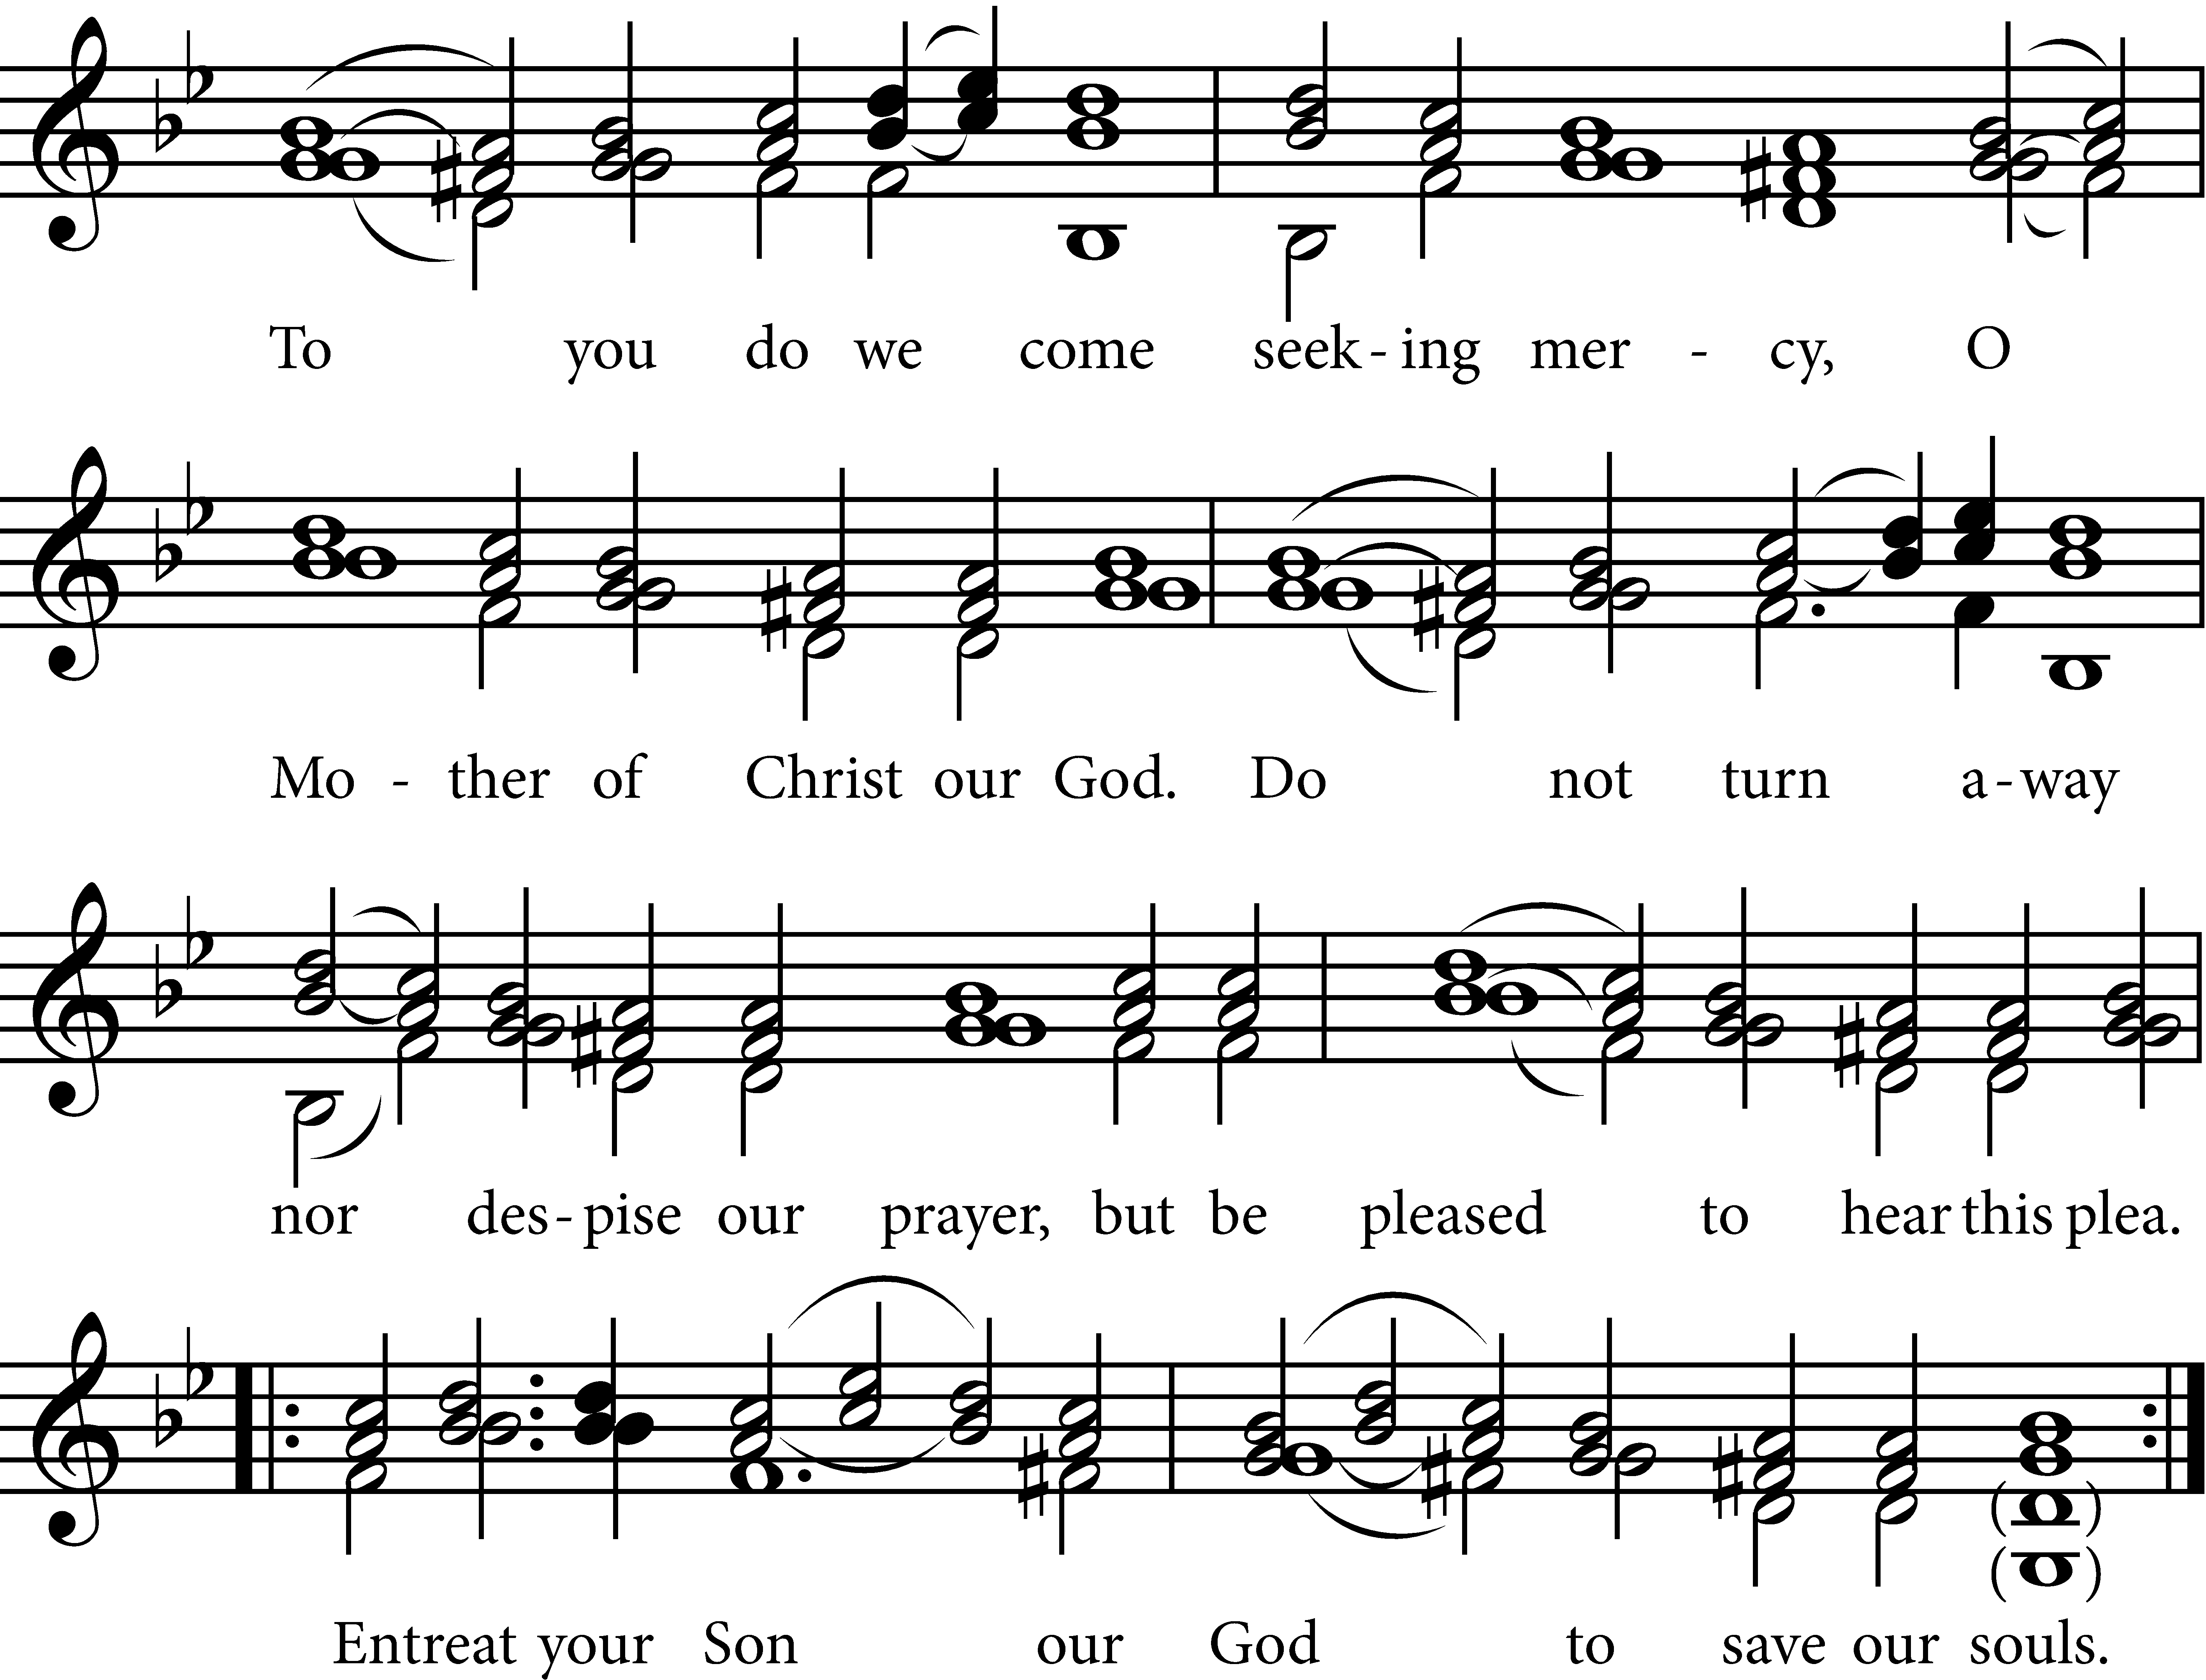
\includegraphics[width=\textwidth]{chants/an--sub_tuum--slavonic.png}\centering\end{figure}  \vspace{5pt} \emph{}  \newpage
  \subsection{Advent}
   \subsubsection{Antiphona}  \greannotation{V} \index[Antiphons]{Alma Redemptoris (Solemn)} \label{Alma Redemptoris (Solemn) (Antiphona)} \grecommentary[5pt]{Ecclesia} \gresetinitiallines{1} \grechangestyle{initial}{\fontsize{36}{36}\selectfont} \grechangedim{maxbaroffsettextleft@nobar}{12 cm}{scalable} \grechangedim{spaceabovelines}{0.5cm}{scalable} \gresetlyriccentering{vowel}   \gregorioscore{chants/an--alma_redemptoris--solemn}  \vspace{5pt} \emph{Loving Mother of the Redeemer, you who remain the open gate of heaven, and the star of the sea, hasten to the aid of your people who, falling, strive to rise again. You who, to the wonderment of nature, bore your holy Creator, remaining a virgin after as before, receiving that ``Ave” from the mouth of Gabriel: have mercy on us sinners.}  \newpage
  \subsection{Advent}
   \subsubsection{Antiphona}  \greannotation{V} \index[Antiphons]{Alma Redemptoris (Simple)} \label{Alma Redemptoris (Simple) (Antiphona)} \grecommentary[3pt]{Ecclesia} \gresetinitiallines{1} \grechangestyle{initial}{\fontsize{36}{36}\selectfont} \grechangedim{maxbaroffsettextleft@nobar}{12 cm}{scalable} \grechangedim{spaceabovelines}{0.5cm}{scalable} \gresetlyriccentering{vowel}   \gregorioscore{chants/an--alma_redemptoris--simple}  \vspace{5pt} \emph{ Loving Mother of the Redeemer, you who remain the open gate of heaven, and the star of the sea, hasten to the aid of your people who, falling, strive to rise again. You who, to the wonderment of nature, bore your holy Creator, remaining a virgin after as before, receiving that ``Ave” from the mouth of Gabriel: have mercy on us sinners.}  \newpage
  \subsection{Lent}
   \subsubsection{Antiphona}  \greannotation{VI} \index[Antiphons]{Ave Regina cælorum (Solemn)} \label{Ave Regina cælorum (Solemn) (Antiphona)} \grecommentary[3pt]{Ecclesia} \gresetinitiallines{1} \grechangestyle{initial}{\fontsize{36}{36}\selectfont} \grechangedim{maxbaroffsettextleft@nobar}{12 cm}{scalable} \grechangedim{spaceabovelines}{0.5cm}{scalable} \gresetlyriccentering{vowel}   \gregorioscore{chants/an--ave_regina--solemn}  \vspace{5pt} \emph{Hail, Queen of Heaven. Hail, Mistress of the Angels. Hail the root, hail the gate, whence came the light of the world. Rejoice, O glorious Virgin, beautiful above all others. Farewell, O fairest one, and pray for us always to Christ.}  \newpage
  \subsection{Lent}
   \subsubsection{Antiphona}  \greannotation{VI} \index[Antiphons]{Ave Regina cælorum (Simple)} \label{Ave Regina cælorum (Simple) (Antiphona)} \grecommentary[0pt]{Ecclesia} \gresetinitiallines{1} \grechangestyle{initial}{\fontsize{36}{36}\selectfont} \grechangedim{maxbaroffsettextleft@nobar}{12 cm}{scalable} \grechangedim{spaceabovelines}{0.5cm}{scalable} \gresetlyriccentering{vowel}   \gregorioscore{chants/an--ave_regina--simple}  \vspace{5pt} \emph{Hail, Queen of Heaven. Hail, Mistress of the Angels. Hail the root, hail the gate, whence came the light of the world. Rejoice, O glorious Virgin, beautiful above all others. Farewell, O fairest one, and pray for us always to Christ.}  \newpage
  \subsection{Easter}
   \subsubsection{Antiphona}  \greannotation{VI} \index[Antiphons]{Regina cæli (Solemn)} \label{Regina cæli (Solemn) (Antiphona)} \grecommentary[0pt]{Ecclesia} \gresetinitiallines{1} \grechangestyle{initial}{\fontsize{36}{36}\selectfont} \grechangedim{maxbaroffsettextleft@nobar}{12 cm}{scalable} \grechangedim{spaceabovelines}{0.5cm}{scalable} \gresetlyriccentering{vowel}  \grechangestyle{translation}{\fontsize{11}{11}\selectfont} \gregorioscore{chants/an--regina_caeli--solemn} \grechangestyle{translation}{\fontsize{10}{10}\it\selectfont} \vspace{5pt} \emph{Queen of heaven, rejoice, alleluia. For he whom you were worthy to bear, alleluia, has risen (ascended) as he said, alleluia. Pray for us to God, alleluia.}  \newpage
  \subsection{Easter}
   \subsubsection{Antiphona}  \greannotation{VI} \index[Antiphons]{Regina cæli (Simple)} \label{Regina cæli (Simple) (Antiphona)} \grecommentary[7pt]{Ecclesia} \gresetinitiallines{1} \grechangestyle{initial}{\fontsize{36}{36}\selectfont} \grechangedim{maxbaroffsettextleft@nobar}{12 cm}{scalable} \grechangedim{spaceabovelines}{0.5cm}{scalable} \gresetlyriccentering{vowel}  \grechangestyle{translation}{\fontsize{11}{11}\selectfont} \gregorioscore{chants/an--regina_caeli--simple} \grechangestyle{translation}{\fontsize{10}{10}\it\selectfont} \vspace{5pt} \emph{Queen of heaven, rejoice, alleluia. For he whom you were worthy to bear, alleluia, has risen (ascended) as he said, alleluia. Pray for us to God, alleluia.}  \newpage
  \section{Chants in Honor of St. Dominic}
   \subsubsection{Responsorium prolixa}  \greannotation{I} \index[Responsories]{O spem miram} \label{O spem miram (Responsorium prolixa)} \grecommentary[3pt]{Ecclesia} \gresetinitiallines{1} \grechangestyle{initial}{\fontsize{36}{36}\selectfont} \grechangedim{maxbaroffsettextleft@nobar}{12 cm}{scalable} \grechangedim{spaceabovelines}{0.45cm}{scalable} \gresetlyriccentering{vowel}   \gregorioscore{chants/rp--o_spem_miram--tp_et_non_tp}  \vspace{5pt} \emph{O wonderful hope, which you gave to those who wept for you at the hour of your death, promising that after your death you would be helpful to your brethren! * Fulfill, Father, what you have said, and help us by your prayers. \Vbar. You shone on the bodies of the sick by so many miracles. Bring us the help of Christ to heal our sick souls. * Fulfill, Father, what you have said, and help us by your prayers.}
   \subsubsection{Antiphona}  \greannotation{I} \index[Antiphons]{Magne Pater} \label{Magne Pater (Antiphona)} \grecommentary[5pt]{Ecclesia} \gresetinitiallines{1} \grechangestyle{initial}{\fontsize{36}{36}\selectfont} \grechangedim{maxbaroffsettextleft@nobar}{12 cm}{scalable} \grechangedim{spaceabovelines}{0.5cm}{scalable} \gresetlyriccentering{vowel}   \gregorioscore{chants/an--magne_pater--compline}  \vspace{5pt} \emph{Great Father, holy Dominic, take us up with you at the hour of our death, and always watch over us lovingly here below.}
   \subsubsection{Antiphona}  \greannotation{I} \index[Antiphons]{Pie Pater} \label{Pie Pater (Antiphona)} \grecommentary[0pt]{Ecclesia} \gresetinitiallines{1} \grechangestyle{initial}{\fontsize{36}{36}\selectfont} \grechangedim{maxbaroffsettextleft@nobar}{12 cm}{scalable} \grechangedim{spaceabovelines}{0.5cm}{scalable} \gresetlyriccentering{vowel}   \gregorioscore{chants/an--pie_pater--compline}  \vspace{5pt} \emph{Loving father, Dominic, be mindful of your works. Stand before the supreme Judge on behalf of your company of poor brothers.}



\chapter{Indices} \thispagestyle{centernumber}

 \printindex[Antiphons]
 \printindex[Hymns]
 \printindex[Responsories]
 \printindex[Varia]




\end{document}
